\documentclass[12pt, a4paper]{report}
\usepackage{graphicx, array, amsthm, amssymb, amsmath, algorithm, algpseudocode, float, xcolor, thmtools, thmbox}
\usepackage[english]{babel}

\makeatletter
\renewcommand\thmbox@headstyle[2]{\bfseries #1}
\makeatother
\newtheorem[style=M,bodystyle=\normalfont]{theorem}{Theorem}
\newtheorem[style=M,bodystyle=\normalfont]{corollary}{Corollary}
\newtheorem[style=M,bodystyle=\normalfont]{lemma}{Lemma}
\newtheorem[style=M,bodystyle=\normalfont]{definition}{Definition}


\title{Uncertainty In Artificial Intelligence \\ \textit{Theory}}
\author{Christian Rossi}
\date{Academic Year 2023-2024}

\begin{document}

\maketitle

\newpage

\begin{abstract}
    The topics of the course are:
    \begin{itemize}
        \item Uncertainty sources that affect models: typology, issues, and modeling approaches.
        \item Measure-based uncertainty modeling.
        \item Logic-based uncertainty modeling.
        \item Fuzzy models: fuzzy sets, fuzzy logic, fuzzy rules, motivations for fuzzy modeling, tools for fuzzy systems, design 
            of fuzzy systems, applications.
        \item Bayesian networks: basics, design, learning, evaluation, applications.
        \item Hidden Markov Models: basics, design, learning, evaluation, applications.
        \item Applications: motivations, choices, models, case studies.
    \end{itemize}
\end{abstract}

\newpage

\tableofcontents

\newpage

\chapter{Introduction}
    \section{Definition}
    \begin{definition}[Uncertainty]
        \emph{Uncertainty} refers to epistemic situations involving imperfect or unknown information. It applies to predictions 
        of future events, to physical measurements that are already made, or to the unknown. 
    \end{definition}
    Uncertainty arises in partially observable or stochastic environments, as well as due to ignorance, indolence, or both. It arises 
    in any number of fields, including insurance, philosophy, physics, statistics, economics, finance, medicine, psychology, sociology, 
    engineering, metrology, meteorology, ecology and information science.
    
    The lack of certainty, a state of limited knowledge where it is impossible to exactly describe the existing state, a future outcome,
    or more than one possible outcome. This puts in evidence that uncertainty is related to the need of describing a piece of reality.

    \section{Modelling}
    Modelling is at the base of our life: the way we interact with the world is through models that interpret data coming from sensors
    and generate knowledge and actions. Modelling is also the way we may represent entities in a computer and possibly making it reasoning
    on them.
    \begin{definition}[Model]
        A \emph{model} is a representation of some entity, defined for a specific purpose. A model captures only the aspects of the entity
        modelled that are relevant for the purpose. A model is necessarily different from the modelled entity. So, intrinsic to modelling
        are all sort of uncertainties.
    \end{definition}
    All Artificial Intelligence applications are based on models, either defined by somebody or learned. These models are represented In
    different ways, but share uncertainty issue mainly on inputs. 

    \section{Uncertainty classification}
    The uncertainty can be of two main types: 
    \begin{itemize}
        \item Epistemic uncertainty: it is due to things one could in principle know but does not in practice. This may because a 
            measurement is not accurate, because the model neglects certain effects, or because particular data have been deliberately
            hidden. It is also known as systematic uncertainty and can in principle be reduced by enriching the model.      
        \item Aleatoric uncertainty: it is representative of unknown unknowns that differ each time we run the same experiment. 
            Aleatoric uncertainty is also known as statistical uncertainty, since only statistical information can describe it. This may
            also depend on the way we get and elaborate data. In general, it is present when the model is missing some aspects.
    \end{itemize}
    The sources of uncertainty can be: 
    \begin{itemize}
        \item Parameter: it comes from the model parameters, whose exact values are unknown to experimentalists and cannot be controlled
            in experiments, or whose values cannot be inferred by statistical methods. 
        \item Parametric variability: it comes from the variability of input variables of the model. 
        \item Structural: also known as model inadequacy, model bias, or model discrepancy, this comes from the lack of knowledge of the
            problem.
        \item Algorithmic: also known as numerical uncertainty, or discrete uncertainty. This type comes from numerical errors and
            numerical approximations in the implementation of the computer model. 
        \item Experimental: also known as observation error, this comes from the variability of experimental measurements.
        \item Interpolation: this comes from a lack of variable data collected from computer model simulations and/or experimental 
            measurements. 
    \end{itemize}

    \section{Uncertainty modelling}
    The type of uncertainty model depends on the type of uncertainty, its sources and the information we have in uncertainty and mostly
    has to do with qualification and quantification of uncertainty. The possible models for uncertainty are: statistical, logical and
    cognitive.

    Artificial Intelligence and Machine Learning technologies are based on models that include uncertainty models of these sorts, essential
    not only for the implementation of effective models, but also to define learning models able to cope with complex situations, and 
    to evaluate the quality of learned/developed models. 
    There are two major types of problems in uncertainty quantification: 
    \begin{itemize}
        \item Forward propagation of uncertainty: the various sources of uncertainty are propagated through the model to predict the overall
            uncertainty in the system response:
            \begin{itemize}
                \item To evaluate low-order moments of the outputs (mean and variance).
                \item To evaluate the reliability of the outputs.
                \item To assess the complete probability distribution of the outputs. 
            \end{itemize}
            This is what is done also in Bayesian networks and graphical models. 
        \item Inverse assessment of model uncertainty and parameter uncertainty, where the model parameters are calibrated simultaneously
            using test data: given some experimental measurements of a system and some results from its mathematical model, inverse 
            uncertainty quantification estimates the discrepancy between the experiment and the mathematical model (bias correction) and
            estimates the values of unknown parameters in the model if there are any (parameter calibration).
    \end{itemize}
    The models used in Artificial Intelligence can be classified in three main types: 
    \begin{itemize}
        \item Symbolic models: elements of the models are expressed as terms related to entities to be modelled. The state of the world is
            represented by facts expressed in formal languages close to natural languages.
        \item Sub-symbolic models: elements of the models are expressed by code. 
        \item Black-box models: the model can be computed and possibly investigated, but it is only regarded as a computational way to map
            inputs to outputs. 
    \end{itemize}
    For symbolic models a fact is true in a model if it is possible to collect enough evidence to support it. The only really true facts 
    are the ones true by definition. All the others may be supported by evidence. 
    
    \section{Ignorance management}
    There are many potential sources of ignorance when reasoning in the real world:
    \begin{itemize}
        \item Insufficient data.
        \item Biased data: data are collected by sensors affected by errors. 
        \item Variable data: data are collected by imprecise sensors.
        \item Reliability of data. 
        \item Fuzzyness. 
        \item Reliability of the model: depends on the model design, implementation and parametrization. 
        \item Incompleteness of the model. 
    \end{itemize}
    \begin{example}
        Let's consider the sentence "The elephant weighs 2 tons". This can be interpreted in various ways, each slightly different:
        \begin{itemize}
            \item The elephant weighs exactly 2 tons.
            \item The elephant weighs 2 tons ± 10 kg, given the resolution of the weight scales of the instrument.
            \item The elephant weighs approximately 2 tons, but we cannot say anything more precise.
            \item We are not sure about any previous sentence because we do not have enough evidence.
        \end{itemize}
    \end{example}
    \begin{figure}[H]
        \centering
        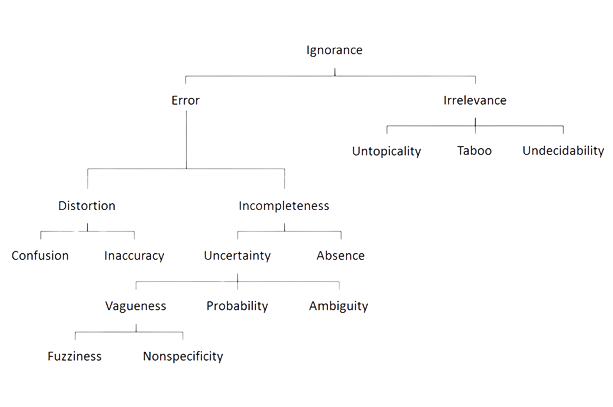
\includegraphics[width=1\linewidth]{images/smithson.png}
        \caption{Smithson's taxonomy of ignorance and uncertainty}
    \end{figure}
    To model ignorance most often it is decided to associate measures of some aspects. Let's distinguish between two aspects: 
    \begin{itemize}
        \item The type of representation: numbers, labels, intervals, \dots
        \item The represented ignorance that we would like to model: i.e, probability, reliability, subjective evaluation, \dots
    \end{itemize}

    The probability is represented with numbers between zero and one, and a well-established set of rules and properties are associated 
    to its management, among which, given a set of alternative hypothesis: 
    \begin{itemize}
        \item The sum of their probabilities should be one. 
        \item The probability a posteriori of a hypothesis $h_i$ given some evidence $e$ is given by the Bayes theorem:
            \[P(h_i \mid e)=\frac{P(e \mid h_i)P(h_i)}{P(e)}\]
    \end{itemize}
    Probability was used, for example, in the MYCIN that was one of the first expert systems, aimed at diagnosing blood illness. They 
    modeled certainty by considering two numerical factors: 
    \begin{itemize}
        \item Measure of increased Belief: $MB=\frac{P(\frac{h}{e})-P(h)}{1-P(h)}$.
        \item Measure of decreased Disbelief: $MD=\frac{P(h)-P(\frac{h}{e})}{P(h)}$.
    \end{itemize}
    The measure of a statement is given by the certain factor:
    \[CF=MB-MD \in [-1;1]\]
    The main hypothesis for this solution is that the number given as $MB$ and $MD$ are not statistical probabilities, but subjective
    probabilities, provided by different experts and combined by rules (this may be ambiguous). 

    Compared to probabilities, linguistic terms are less ambiguous than numbers. Using a limited set of labels it is possible to associate
    to statements subjective evaluation, on which it is relatively easy to make subjective judgements converge. Then, a computational 
    mechanism is needed to define how to combine labels. This is done by using fuzzy systems, that are a representation of truth  of a 
    statement in linguistic terms, as evaluation of its fuzzyness. 
    
    \newpage

    \chapter{Fuzzy sets}
    \section{History}
    Fuzzy sets have been defined by Lotfi Zadeh in 1965 as a tool to model approximate concepts. In 1972 the first linguistic fuzzy
    controllers has been implemented. Around 1980 the fuzzy were used frequently worldwide. In the Nineties there were a massive 
    diffusion of fuzzy controllers in various end-user goods. Today, fuzzy systems are the kernel of many intelligent devices. 

    \section{Fuzzy membership function}
    A "crisp" set is defined by a boolean membership function on some property on the considered elements. Instead, a "fuzzy" set is
    a set whose membership function that ranges in the values between zero and one.
    \begin{definition}[Membership function]
        A \emph{membership function} defines a set, by defining the degree of membership of an element of the universe of discourse 
        to the set. A name is given to the set to make it possible to refer to it: this is usually called \emph{label}. Fuzzy sets can 
        also be defined with a variable with discrete values. 
    \end{definition}
    \begin{figure}[H]
        \centering
        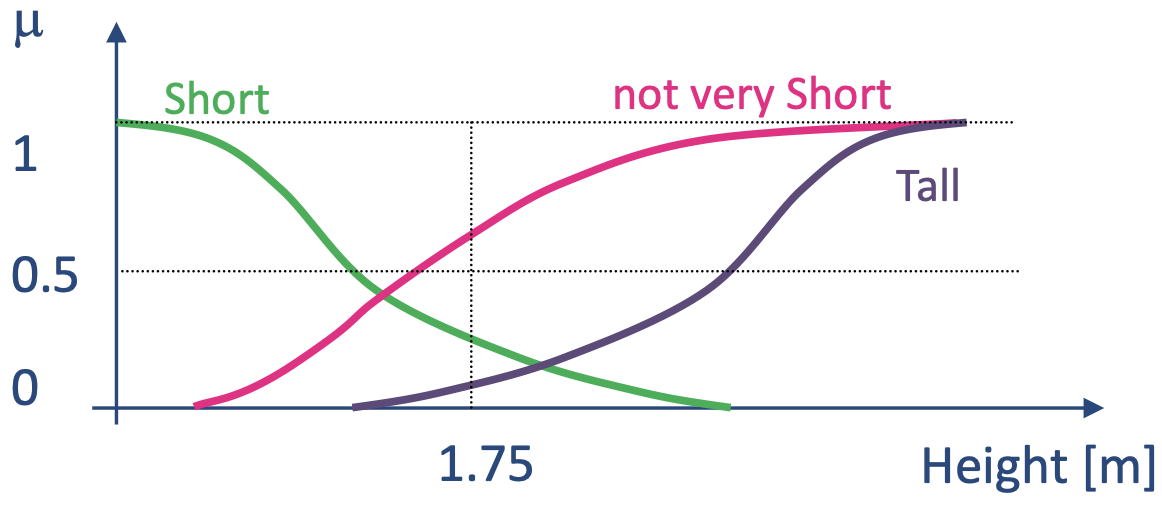
\includegraphics[width=0.50\linewidth]{images/function.png}
        \caption{Example of a membership function}
    \end{figure}
    To define a membership function we have to (according to the purpose of the model and the available data):
    \begin{enumerate}
        \item Select a variable on which the membership function will be defined. 
        \item Define the range of the variable.
        \item Identify the fuzzy sets needed for the application and define the labels. 
        \item For each fuzzy set identify characteristic points for the membership function.
        \item Define the shape of the membership function.
        \item Check if the membership function is correct.
    \end{enumerate}
    The shapes of the membership function can be chosen arbitrarily. The choice of the shape modify the smoothness of the transition 
    between two labels (i.e., in intervals (horizontal shape) the transition is immediate). 
    \begin{figure}[H]
        \centering
        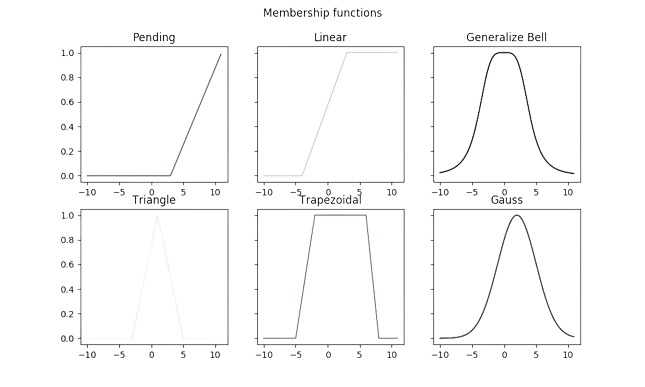
\includegraphics[width=0.75\linewidth]{images/shape.png}
        \caption{Possible shapes for a membership function}
    \end{figure}
    \begin{definition}
        A set of fuzzy sets fully covering the universe of discourse is called \emph{frame of cognition}. The properties of this set are:
        \begin{itemize}
            \item Coverage: each element of the universe of discourse us assigned to at least one granule with membership greater or equal 
                than zero.
            \item Uni-modality of fuzzy sets: there is a unique set of values for each granule with maximum membership. 
        \end{itemize}
    \end{definition}
    \begin{definition}
        A frame of cognition for which the sum  of the membership values of each value of the base variable is equal to one is called 
        a \emph{fuzzy partition}. 
    \end{definition}
    \begin{definition}
        The \emph{$\alpha$-cut} of a fuzzy set is the "crisp" set of the values of $x$ such that $\mu(x) \geq \alpha$:
        \[\alpha_\mu(x)=\{x \mid \mu(x) \geq \alpha\}\]
    \end{definition}
    \begin{figure}[H]
        \centering
        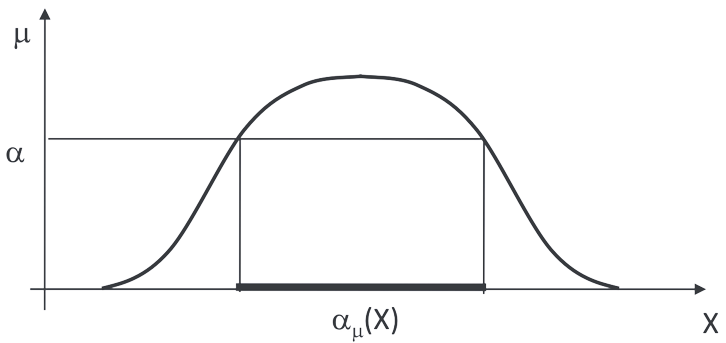
\includegraphics[width=0.5\linewidth]{images/alpha.png}
        \caption{Alpha-cut of a membership function}
    \end{figure}
    \begin{definition}[H]
        The \emph{support} of a fuzzy set is the "crisp" set of values $x$ such that $\mu_f(x)>0$ is the \emph{support} of the fuzzy set
        $f$ on the universe $X$.
    \end{definition}
    \begin{figure}[H]
        \centering
        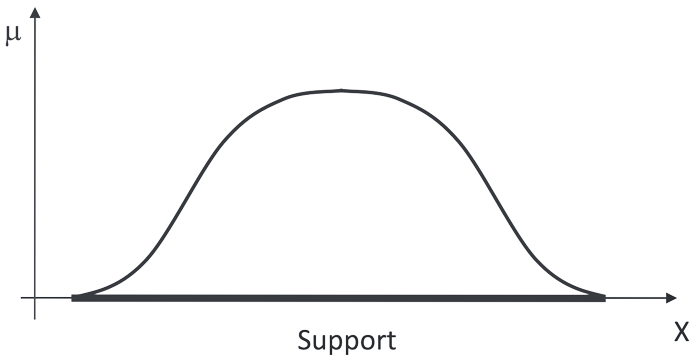
\includegraphics[width=0.5\linewidth]{images/support.png}
        \caption{Support of a membership function}
    \end{figure}
    \begin{definition}
        The height $h_f$ of a fuzzy set $f$ on the universe $X$ is the highest membership degree of an element of $X$ to the fuzzy set:
        \[h_f(X)=\max_{x \in X}\mu_f(x)\]
        A fuzzy set is normal if, and only if, $h_f(X)=1$.
    \end{definition}
    \begin{figure}[H]
        \centering
        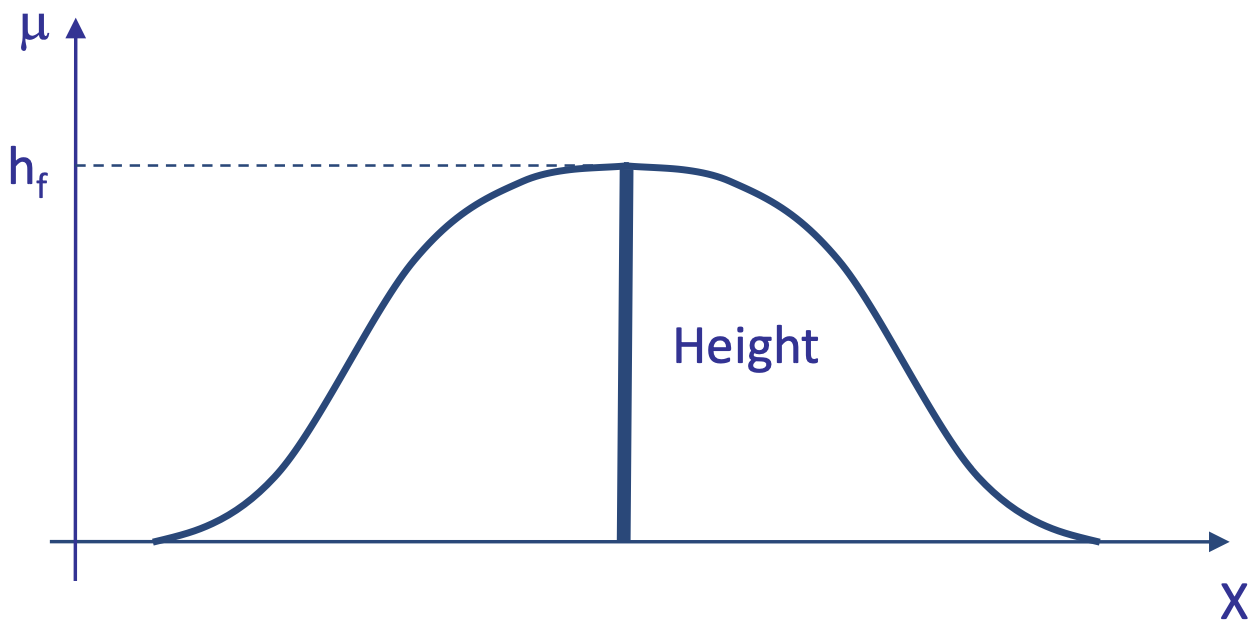
\includegraphics[width=0.5\linewidth]{images/height.png}
        \caption{Height of a membership function}
    \end{figure}
    \begin{definition}
        A fuzzy set is \emph{convex} if and only if 
        \[\mu[\lambda x_1+(1-\lambda)x_2] \geq \min [\mu(x_1),\mu(x_2)]\]
        for any $(x_1,x_2) \in \mathbb{R}$ and any $\lambda \in [0,1]$.
    \end{definition}
    \begin{figure}[H]
        \centering
        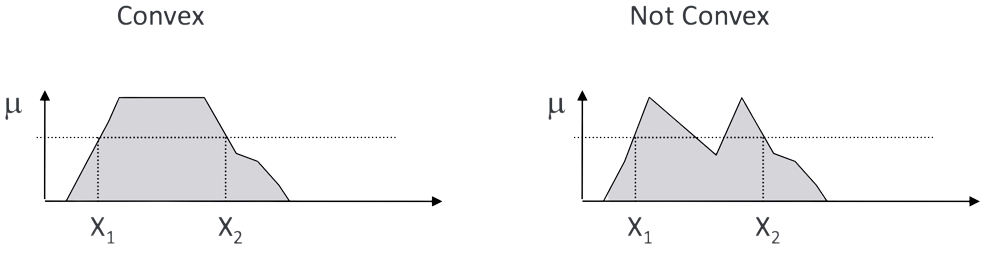
\includegraphics[width=0.75\linewidth]{images/convex.png}
        \caption{Graphical difference between a convex and a not convex set}
    \end{figure}
    The particular fuzzy sets are: singleton (a fuzzy set with exactly one member) and interval (a fuzzy set whose members have all membership
    equals to one). The possible operations on the fuzzy sets are: 
    \begin{itemize}
        \item Complement: $\mu_{\bar{f}}(x)=1-\mu_f(x)$.
        \item Union: $\mu_{f_1 \cup f_2}(x)=\max [\mu_{f_1}(x),\mu_{f_2}(x)]$.
        \item Intersection: $\mu_{f_1 \cap f_2}(x)=\min [\mu_{f_1}(x),\mu_{f_2}(x)]$.
    \end{itemize}

    \newpage

    \chapter{Fuzzy logic}
    \section{Introduction}
    Logic is a tool that has been used since a thousand of years to formally represent knowledge. There are many types of logic: 
    \begin{itemize}
        \item Propositional: truth values for proposition.
        \item First order: truth values for predicates (with variables and quantifiers).
        \item Second order: predicates of predicates.
    \end{itemize}
    These types of logic are binary. We may notice that the meaning of the terms in these logics is not defined together with the formalism,
    and this is not needed to make the logic work.

    \section{Propositional logic}
    Propositional logics are concerned with propositional operators which may be applied to one or more propositions giving new propositions.
    The accent is on the truth value of propositions and on how these truth values are composed.
    \begin{definition}
        A logic is \emph{truth functional} if the truth value of a compound sentence depends only on the truth values of the consistent atomic 
        sentences, not on their meaning or structure. For such a logic the only important question about propositions is what truth values may
        have.
    \end{definition}
    In a classical, boolean or two-valued logic every proposition is either true or false and no other feature of the proposition is relevant.

    The main operators in the propositional logics are: conjunction ($\land$), disjunction ($\lor$) and negation ($\lnot$).

    \section{First order predicate logic}
    The first order logic is the same as propositional logic augmented with the possibility to define predicates on variables. Furthermore, 
    existential ($\exists$) and universal ($\forall$) quantifiers are defined. 
    In predicate logics it is possible to infer the truth value of a proposition by inferential mechanisms, such as Modus Ponens. 
    \begin{example}[Inference]
        Given the sentences: "All man are mortal" and "Socrates is a man" we can infer that "Socrates is mortal".
    \end{example}
    Inference is used to model a mechanism that we have in our minds to store a reduced amount of information and set a mechanism that can be 
    applied to derive from information other information, to face everyday situations.
    \begin{definition}
        Information and potential relationship together compose what we call \emph{knowledge}.
    \end{definition}
    
    \section{Many-valued logics}
    Aristotle already had put in evidence problems about the validity of classical logic as a knowledge representation tool. For instance, it is
    difficult to state the truth value of a proposition in the future. To solve this problem, let's introduce a third value (i.e., 0.5) for the 
    undefined situation and define a three-valued logic. From this to an infinite set of truth values there is just a small step.
    
    Infinite-value logics considers a continuum of truth values between zero and one for example. 

    \begin{example}[Logic L1, Łukasiewicz(1930)]
        The main rules in this type of infinite-value logic are: 
        \begin{itemize}
            \item $T(\lnot a)=1-T(a)$.
            \item $T(a \land b)=\min (T(a),T(b))$.
            \item $T(a \lor b)=\max (T(a),T(b))$.
            \item $T(a \implies b)=\min (1, 1+T(b)-T(a))$.
            \item $T(a \Leftrightarrow b)=1-\left\lvert T(a)-T(b) \right\rvert$.
        \end{itemize}
    \end{example}

    This innovations bring a change in the society: things are no longer stated as true or false, probability (kolmogorov, 1929) and 
    stochasticity (Markov, 1906) became the way to represent the new approach to science and life. 

    The difference between classical logic L2 and many-valued logic L1 are the following: 
    \begin{itemize}
        \item L1 is isomorphic to the fuzzy set theory with standard operators as the classical logic L2 is isomorphic to the set theory.
        \item Tautologies are true by definition, and are used to prove theorems, so to prove the truth of an inferential chain. 
            Some tautologies valid in L2 are no longer valid in L1, for example:
            \begin{itemize}
                \item Third excluded law ($T(a \lor \lnot a)=1$)
                \item Non-contradiction law ($T(a \land \lnot a)=0$).
            \end{itemize}
    \end{itemize}

    The sentence "I'm a liar" would be a paradox in classical logic, if we give a meaning to the term "liar", since no formula can have the
    same truth value of its negation. This may not be so in many-valued logics. In Łukasiewicz logic, for instance, it can be that the truth 
    value of a sentence is 0.5, and that its negation is the same, so the proposition is consistent with the axioms, and it is not a paradox. 

    \section{Fuzzy logic}
    Fuzzy logic is an infinite-valued logic, with truth values in $[0 \dots 1]$ and prepositions are expressed as: 
    \[A \: is \: L\]
    where: 
    \begin{itemize}
        \item $A$ is a linguistic variable.
        \item $L$ is a label denoting a fuzzy set.
    \end{itemize}

    Formally, a linguistic variable is defined by a 5-tuple $(X,T(X),U,G,M)$, where: 
    \begin{itemize}
        \item $X$ is the name of the variable.
        \item $T(X)$ is the set of term for $X$, each corresponding to a fuzzy variable denoted by $T(X)$ and ranging on $U$.
        \item $U$ is the universe of discourse defined on a base variable $u$.
        \item $G$ is the syntactic rule used to generate the interpretation $X$ of each value $u$.
        \item $M$ is the semantic rule used to associate to $X$ its meaning.
    \end{itemize}
    \begin{example}[Linguistic variable for age]
        We can define a linguistic variable for the age in the following way:
        \begin{itemize}
            \item $X$ is a linguistic variable labelled "age".
            \item $U=[0 \dots 100]$.
            \item $T(X)={old, middle-aged, young, \dots}$.
            \item $u=[0 \dots +\infty]$.
            \item $M$ is the definition in terms of fuzzy sets of the values of $X$.
            \item $G$ is the fuzzy matching interpretation of $u$.
        \end{itemize}
    \end{example}

    Now that we have defined the linguistic variable it is possible to write a simple proposition in the following way: 
    \[p\: : \: X \: is \: F\]
    where:
    \begin{itemize}
        \item $X$ is a linguistic variable.
        \item $F$ is the label of a fuzzy set, defined on $U$, which represent a fuzzy predicate.
        \item $\mu_F(x)$ is the membership function defining $F$, and it is interpreted as truth value for the preposition $p$ ($T(p)=\mu_F(x)$).
    \end{itemize}
    Therefore, the truth value of the preposition $P$ is a fuzzy set defined on $[0 \dots 1]$.
    \begin{example}
        Given the simple proposition "p:temperature is high", where $X$ is temperature and $F$ is high we can find the truth value of this 
        preposition using the graph of the membership function given:
        \begin{figure}[H]
            \centering
            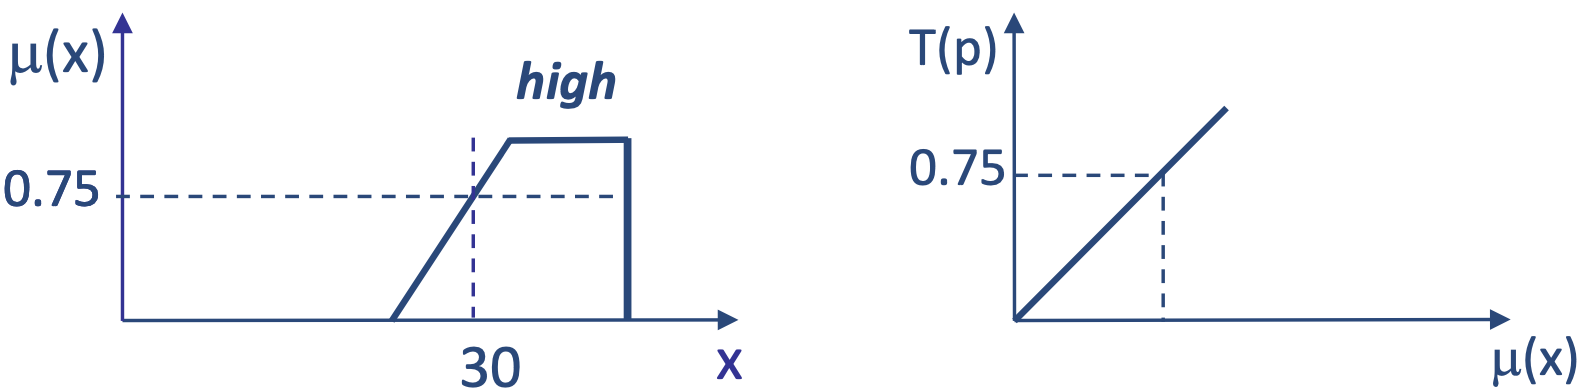
\includegraphics[width=0.5\linewidth]{images/temperature.png}
        \end{figure}
        So, the truth value of the given proposition is $0.75$.
    \end{example}

    It is also possible to define qualified, non-conditional propositions with this syntax: 
    \[p \: : \: (X \: is \: F) \: is \: S\]
    where:
    \begin{itemize}
        \item $S$ is a fuzzy truth qualifier.
        \item $F$ is a fuzzy set.
        \item $p$ is truth qualified.
    \end{itemize}
    \begin{example}
        Given the conditional proposition "p:age of Tina is young is very true", where $X$ is age, $F$ is young and $S$ is very true we can 
        find the truth value of this preposition using the graph of the membership function given:
        \begin{figure}[H]
            \centering
            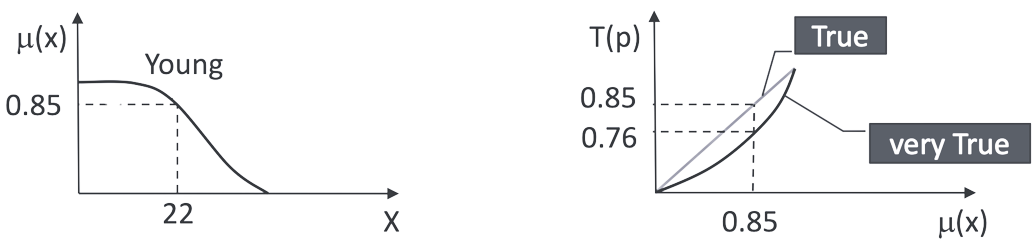
\includegraphics[width=0.75\linewidth]{images/age.png}
        \end{figure}
    \end{example}

    In the fuzzy logic it is possible to use fuzzy modifiers to modify the truth values of the propositions.     
    The modifiers can be of two main types: 
    \begin{itemize}
        \item Strong ($m(a) \leq a \: \forall a \in [0 \dots 1]$): they make the predicate stronger, so they reduce the truth of the preposition.
        \item Weak($m(a) \geq a \: \forall a \in [0 \dots 1]$): they make the predicate weaker, so they increase the truth of the preposition.
    \end{itemize}
    The properties of the fuzzy modifiers are:
    \begin{itemize}
        \item $m(0)=0$ and $m(1)=1$.
        \item $m$ is a continuous function. 
        \item If $m$ is strong $m^{-1}$ is weak, and the other way around.
        \item Given another modifier $g$, the composition of $g$ and $m$ and the other way round are modifiers, too, and, if both are strong
            (or weak), so it's their composition.
    \end{itemize}
    \begin{example}
        The sentence "x is young" actually means "(x is young) is true". This sentence can be modified in the following ways with fuzzy modifiers:
        \begin{itemize}
            \item "x is very young is true".
            \item "x is young is very true".
            \item "x is very young is very true". 
        \end{itemize}
        Graphically we can draw the modified membership function as: 
        \begin{figure}[H]
            \centering
            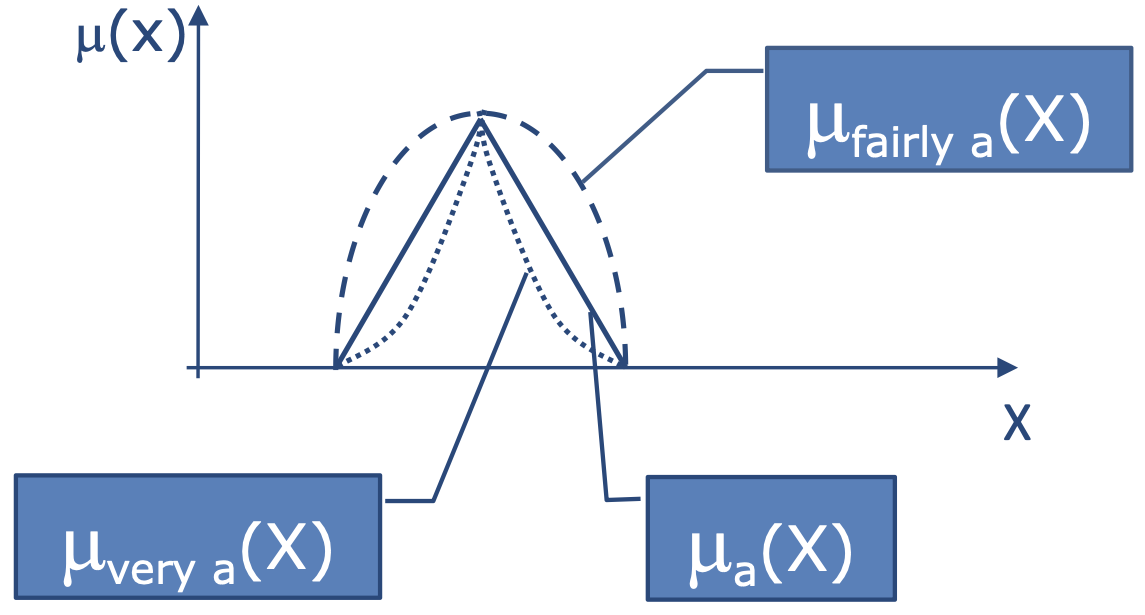
\includegraphics[width=0.4\linewidth]{images/modifiers.png}
        \end{figure}
        where: 
        \begin{itemize}
            \item $\mu_{very \: a}(x)=\mu_a(x)^2$.
            \item $\mu_{fairly \: a}(x)=\mu_a(x)^{\frac{1}{2}}$.
        \end{itemize}
    \end{example}

    \section{Inference rules}
    \begin{definition}
        An \emph{inference rule} is a model. In other words it is a way to define a mapping from input to output. 
        Rules are used to represent inferential relationships among pieces of knowledge.
    \end{definition}
    We consider forward chaining rules, having the shape:
    \[IF \: antecedent \: THEN \: consequent\]
    where:
    \begin{itemize}
        \item $antecedent$ is a set of clauses related by logical operators.
        \item $consequent$ is a set of clauses related by logical operators.
    \end{itemize}
    The clauses used in the inference rules are either a proposition (sequence of symbols) or a pattern (sequence of symbols and variables). 

    Inference rules are used to implement Knowledge-Based Systems, among which Expert Systems are mostly known as successful Artificial
    Intelligence applications. An Expert System is designed upon the experience of somebody to replicate, or improve his performance in solving
    a problem. Knowledge Acquisition is a complex process bringing to the definition of rule-based systems, implemented and running on computers.

    A system can generate new information using rules and other related information using these steps:
    \begin{enumerate}
        \item Pattern matching: identify the rules whose antecedents match the known facts (saved in the fact base). These can be considered for
            activation, given the corresponding assignment to variables.
        \item Selection of the rules to be activated: among the rules identified with pattern matching (candidate rules), select the rules that
            should be activated.
        \item Activation of the selected rules: assert the consequent of the selected rules in the fact base. 
    \end{enumerate}
    \begin{example}
        Suppose that the rule base contains the following four rules:
        \begin{enumerate}
            \item "If X croaks and X eats flies, then X is a frog".
            \item "If X chirps and X sings, then X is a canary".
            \item "If X is a frog, then X is green".
            \item "If X is a canary, then X is yellow".
        \end{enumerate}
        Now suppose to observe the following facts (fact base):
        \begin{itemize}
            \item Fritz croaks.
            \item Fritz eats flies.
        \end{itemize}
        From rule 1 and facts a and b we can add to the fact base the fact: 
        \[Fritz \: is \: a \: frog\]
        Given the new fact base, we can use rule 3 to deduce the fact: 
        \[Fritz \: is \: green\]
    \end{example}

    \section{Fuzzy rules}
    \begin{definition}
        A \emph{fuzzy rule} is a rule whose clauses have the shape
        \[(V \: is \: L)\]
        where $V$ is a linguistic variable and $L$ is a label, a value for $V$ associated to a fuzzy set. This is a \emph{linguistic clause}.
    \end{definition}
    Often, clauses in the antecedent are only related by the AND operator which is not explicitly written. 
    The antecedent is usually matched against facts that are represented as values of the base variables corresponding to the linguistic variables.
    The consequent may be one of two types:
    \begin{itemize}
        \item Linguistic rules: the consequent is a conjunction of linguistic clauses. These rules can be considered as a mapping between
            the interpretation of an input configuration and a symbolic description of the desired output. The general formula is:
            \[IF \: (A \: is \: LA_i) \: AND \: (B \: is \: LB_k) \: AND \: \dots \: THEN \: (U \: is \: LU_m) \: AND \: \dots\]
        \item Model rules: bind a model to the linguistic interpretation of its applicability conditions. This can be considered as a mapping 
            between the interpretation of an input configuration and a model to be applied to the input real values to obtain the output. 
            The general formula is:
            \[IF \: (A \: is \: LAn) \: AND \: (B \: is \: LBk) \: AND \: \dots \: THEN \: U \: is \: f(A,B)\]
    \end{itemize}
    The steps to use the fuzzy rules are the following: 
    \begin{enumerate}
        \item Input matching.
        \item Combination of matching degrees.
        \item Combination with rule weight, if present.
        \item Aggregation of output from different rules. 
        \item Eventual defuzzyfication of output.
    \end{enumerate}
    To defuzzyficate the output it is possible to consider various operators other than the weighted mean, for example: centroid, bisector,
    average of maxima, the lowest maximum, the highest maximum, center of the highest area, \dots Depending on the choice the system change the 
    output and the level of optimization. 
    \begin{example}[Linguistic rules]
        Let's consider:
        \begin{itemize}
            \item Two input variables (fuzzy partition) $A$ and $B$ equally distributed from Negative Large to Positive Large. 
            \item One output variable $U$ (equally distributed fuzzy set) from Negative Large to Positive Large. The fuzzy sets are all singletons.
        \end{itemize} 
        \begin{figure}[H]
            \centering
            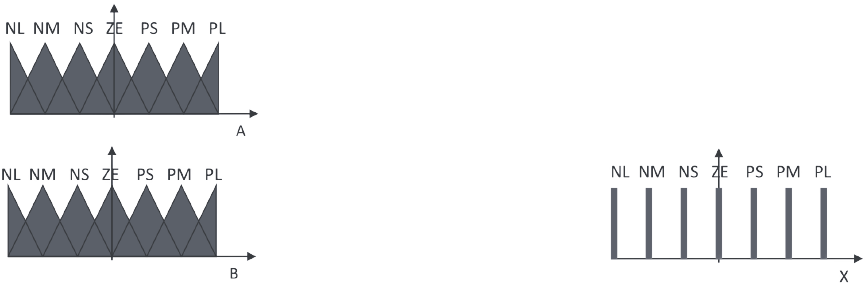
\includegraphics[width=0.75\linewidth]{images/rules.png}
        \end{figure}
        We now have to define the rules of the rule base (each one with a weight) as follows: 
        \begin{enumerate}
            \item IF $A$ is $PL$ AND $B$ is $PS$ THEN $X$ is $PM$ (weight 1).
            \item IF $A$ is $PM$ AND $B$ is $PS$ THEN $X$ is $PS$ (weight 0.5).
            \item IF $A$ is $PL$ AND $B$ is $PM$ THEN $X$ is $PM$ (weight 1).
        \end{enumerate}

        Let's now set $A=22$ and $B=140$. The steps used to calculate the output value are the following:
        \begin{enumerate}
            \item For the first step we have to check the corresponding value for each label. In this case we have:
                \begin{itemize}
                    \item ($A$ is $PL$) has a truth value of $0.2$.
                    \item ($B$ is $PS$) has a truth value of $0.6$.
                    \item ($A$ is $PM$) has a truth value of $0.8$.
                    \item ($B$ is $PM$) has a truth value of $0.4$.
                \end{itemize}
            \item To consider the degree of truth of each predicate we simply take the minimum between the two values (because there is an AND 
                operator). So, the result will be $0.2$ for the first rule, $0.6$ for the second and $0.4$ for the third one.
            \item Now we have to consider the rule weight. To do so we simply select the minimum between the selected value and the weight value.
                So the final value for the consequent are: $0.2$ for the first rule, $0.5$ for the second and $0.4$ for the third one. 
            \item  Now we have to aggregate the output. If we have a repeated expression we take the maximum value between the possible ones. 
                In this case we obtain that ($X$ is $PM$) has a truth value of $0.4$ (maximum between $0.2$ and $0.4$) and ($X$ is $PS$) has a 
                truth value of $0.5$. This result can be visualized graphically by cutting the initial graph as follows.
                \begin{figure}[H]
                    \centering
                    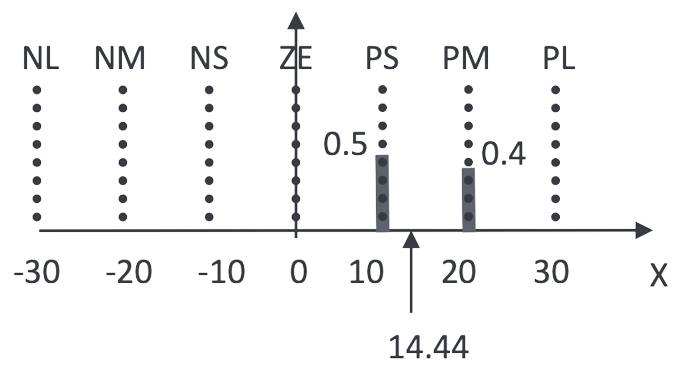
\includegraphics[width=0.5\linewidth]{images/cut.png}
                \end{figure}
            \item Now we can defuzzyficate the result by obtaining a number. We need to do this operation because the input is a number and the 
            desired output needs to be a number. To calculate the exact value of the output it is possible to use a simple weighted mean: 
            \[X=\frac{10 \cdot 0.5 + 20 \cdot 0.4}{0.5+0.4}=14.44\]
        \end{enumerate}
    \end{example}
    \begin{example}[Model rules]
        The variables are the same as the previous example. The rules we are going to consider are the following: 
        \begin{enumerate}
            \item IF $A$ is $PL$ and $B$ is $PS$ THEN $X$ is $A+2B$.
            \item IF $A$ is $PM$ and $B$ is $PS$ THEN $X$ is $A+3$. 
            \item IF $A$ is $PL$ and $B$ is $PM$ THEN $X$ is $A+B$.
        \end{enumerate}
        The models considered in these rules are all linear. Pattern matching is the same as the previous example, and so we have that the 
        subsequent have the following degree of truth: the first one has a value of $0.2$, the second a value of $0.5$ and the third a value of
        $0.4$. For the output aggregation we consider again the weighted mean and use the initial value of $A=22$ and $B=140$ in the resulting 
        formula:
        \[X=\frac{0.2 \cdot (A+2B)+0.5 \cdot (A+3)+ 0.4 \cdot (A+B)}{0.2+0.5+0.4}=125.18\]
    \end{example}

    \section{Fuzzy system design}
    To design a fuzzy system we have to follow those steps:
    \begin{enumerate}
        \item Problem definition.
        \item Parametrization of the model: concepts.
        \item Mapping definition: rules.
        \item Implementation.
        \item Testing.
    \end{enumerate}
    In the problem definition phase we have to choose all the input and output variables and the goal of the model. In principle, input variables
    are numerical or ordinal (like colors) variables so that it is possible to define fuzzy sets on them. Variables can be either: 
    \begin{itemize}
        \item Perceived values coming directly from sensors, data, or users. 
        \item Computed from perceived variables. 
    \end{itemize}
    The selection of the variables is up to designers, so there aren't best or worst input variables to select. Output variables are the result
    of the models, so come directly from the modeler needs. The goals of the fuzzy models depend on the specification. The goals should always be
    stated in advance and guide the design. 

    The system parametrization is based on:
    \begin{itemize}
        \item Selection of the membership functions for all variables. These function can be defined by a:
            \begin{itemize}
                \item Single expert, with objective evaluation or interviews.
                \item Multiple expert, which is more reliable.
                \item Automatic systems working on data (like Neural Networks).
            \end{itemize}
            The number of membership functions for each variable varies between three and seven. 
            Any point in the range of input variables has to be covered by at least one fuzzy set participating to at least one rule and boundaries
            should be covered with maximum value. 
        \item Selection of the inferential mechanism. The inferential engine depends on the operators selected for:
            \begin{itemize}
                \item AND of antecedent clauses (minimum: the worst degree of matching is the most relevant; product: all the degrees of matching
                    are relevant).
                \item Detachment: combination with the rule weight (minimum or product).
                \item Aggregation of the degrees of the same consequent (max: the best degree is the most relevant; probabilistic sum: all the
                    knowledge is considered).
            \end{itemize}
        \item Selection of eventual fuzzyfication and defuzzyfication. 
    \end{itemize}

    The rules can be defined:
    \begin{itemize}
        \item From experience.
        \item From another model.
        \item By using Machine Learning, or self-tuning techniques (like Neural Networks).
    \end{itemize}

    The testing can be done with: dynamic simulation, static simulation or directly on the process, possibly under safe conditions. 

    \section{Applications of fuzzy systems}
    The fuzzy controls are systems able to control the behavior of another system. In most cases it is a PID controller, where the output
    depends on the difference between the desired and the observed behavior. 
    \begin{figure}[H]
        \centering
        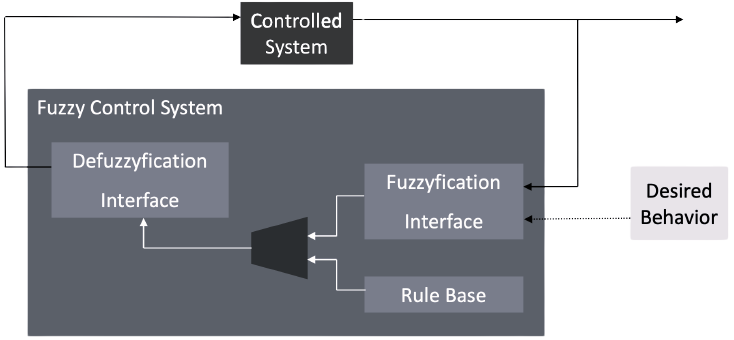
\includegraphics[width=0.5\linewidth]{images/control.png}
        \caption{General schema of a fuzzy control system}
    \end{figure}
    The main features of a fuzzy control system are: 
    \begin{itemize}
        \item Robustness with reference to noise.
        \item Control rules defined over a wide range of applicability.
        \item Possibility to model heuristics from experts.
        \item Smoothness of action.
        \item Non-linearity.
    \end{itemize}

    The fuzzy system can also be used to make database queries that are flexible with human like sensibility. For example with fuzzy sets it
    is possible to make queries like "Give me the names of the people that have recently invested a lot" and give a meaning to "recently" and 
    "a lot". 

    The fuzzy systems can be also used in Artificial Intelligence systems like Expert Systems, scheduling, and Decision Support Systems.

    \newpage

    \chapter{Evidence theory}
    \section{Fuzzy mathematics}
    Fuzzy numbers are fuzzy sets defined over the set of real numbers, which model our concept of approximate value. The constraints used to 
    define fuzzy numbers are: 
    \begin{enumerate}
        \item Normal fuzzy sets.
        \item Convex fuzzy sets (all $\alpha$-cut intervals should be closed).
        \item The support of A should be bounded. 
    \end{enumerate}
    The first constraint captures the concept of approximate value corresponding to a number. The other two constraints are needed to define 
    arithmetic. 

    With fuzzy sets it is possible to define fuzzy numbers (first graph), fuzzy intervals (second graph), defined intervals (third graph) and 
    crisp numbers (fourth graph). 
    \begin{figure}[H]
        \centering
        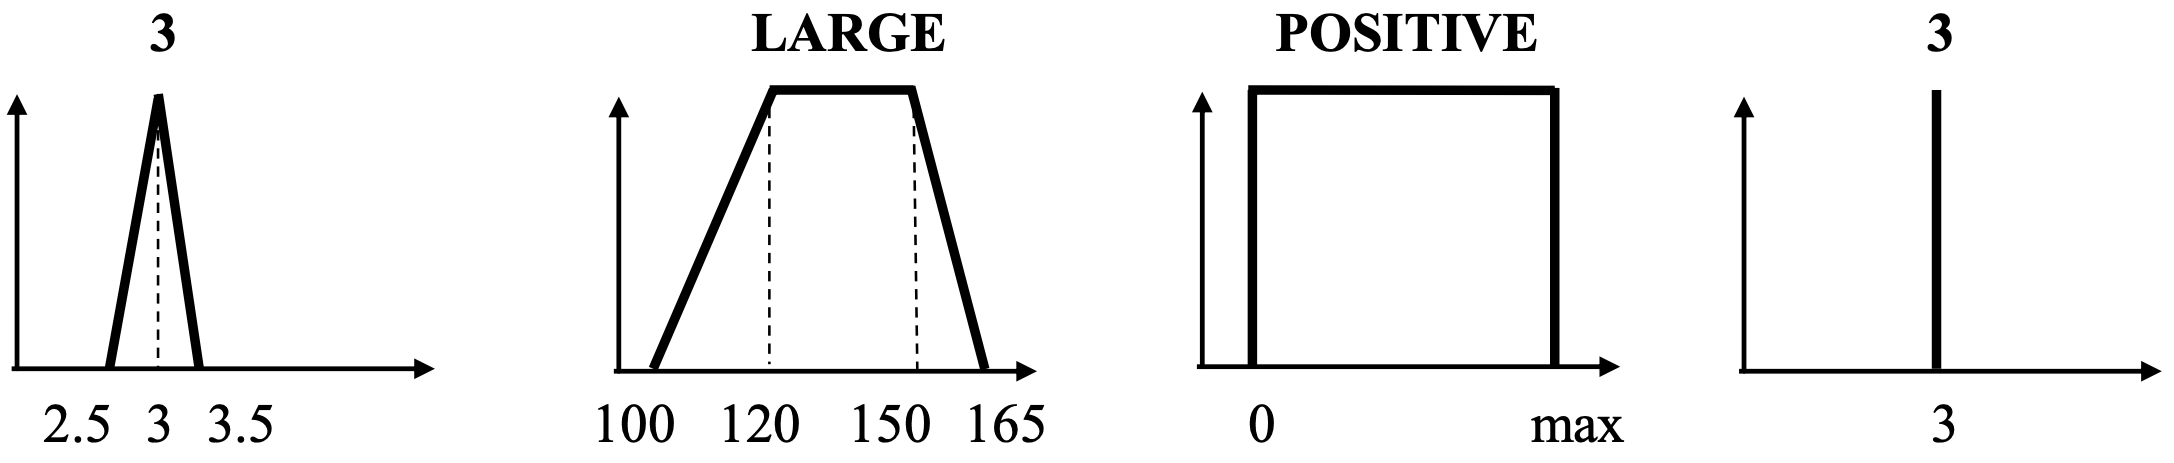
\includegraphics[width=0.75\linewidth]{images/numbers.png}
        \caption{Possible representation of numbers}.
    \end{figure}

    The arithmetic of fuzzy numbers is based on two properties:
    \begin{itemize}
        \item Each fuzzy number can be completely represented by its $\alpha$-cuts uniquely. 
        \item The $\alpha$-cuts of fuzzy numbers are closed intervals of real numbers. 
    \end{itemize}

    The four main operators are defined as the union of the operations on intervals ($\alpha$-cut) that compose the fuzzy number and are: 
    \begin{itemize}
        \item $[a,b]+[d,e]=[a+d,b+e]$.
        \item $[a,b]-[d,e]=[a-e,b-d]$.
        \item $[a,b] \times [d,e]=[\min (ad,ae,bd,be),\max (ad,ae,bd,be)]$
        \item $[a,b] \div [d,e]=[\min (\frac{a}{d},\frac{a}{e},\frac{b}{d},\frac{b}{e}),\max (\frac{a}{d},\frac{a}{e},\frac{b}{d},\frac{b}{e})]$ with $[d,e] \neq [0,0]$
    \end{itemize}

    \begin{example}
        Given the fuzzy numbers $[1,3]$ and $[4,6]$ we have that:
        \begin{itemize}
            \item The sum of the numbers is given by the sum of the minimum and the maximum of each interval:
                \[[1,3]+[4,6]=[1+4,3+6]=[5,9]\]
                Graphically, we obtain the following graph:
                \begin{figure}[H]
                    \centering
                    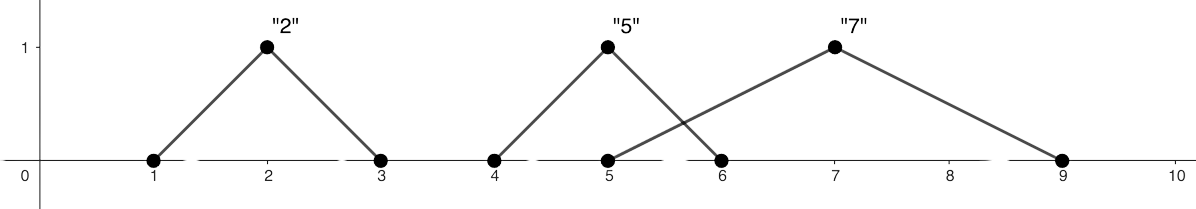
\includegraphics[width=0.75\linewidth]{images/sum.png}
                \end{figure}
            \item The subtraction of the numbers is given by the subtraction of the minimum of the first interval with the maximum of the 
            second and the subtraction of the maximum of the first interval with the minimum of the second interval:
                \[[1,3]+[4,6]=[1-6,3-4]=[-5,-1]\]
                Graphically, we obtain the following graph:
                \begin{figure}[H]
                    \centering
                    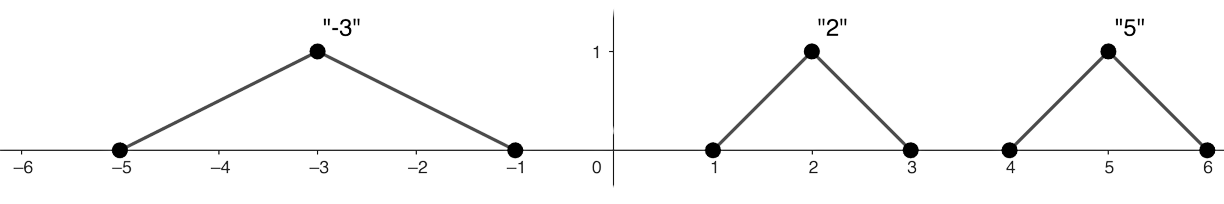
\includegraphics[width=0.75\linewidth]{images/subtraction.png}
                \end{figure}
            \item The multiplication of the numbers is given by the minimum and the maximum of the multiplication of each element:
                \[[1,3] \times [4,6]=[\min(1 \cdot 4, 1 \cdot 6, 3 \cdot 4, 3 \cdot 6),\max(1 \cdot 4, 1 \cdot 6, 3 \cdot 4, 3 \cdot 6)]=[4,18]\]                Graphically, we obtain the following graph:
                \begin{figure}[H]
                    \centering
                    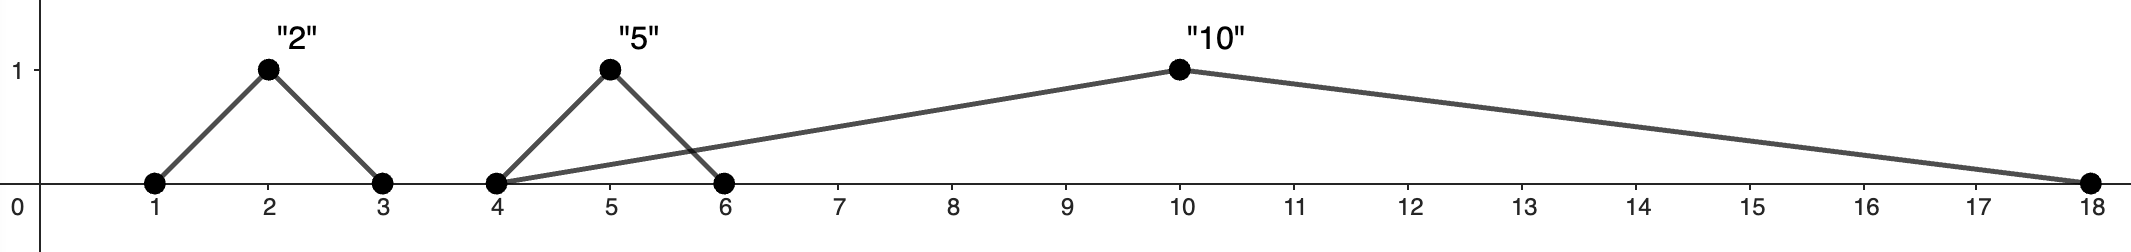
\includegraphics[width=0.75\linewidth]{images/multiplication.png}
                \end{figure}
            \item The division of the numbers is given by the minimum and the maximum of the division of each element:
            \[[1,3] \times [4,6]=[\min(\frac{1}{4}, \frac{1}{6}, \frac{3}{4}, \frac{3}{6}),\max(\frac{1}{4}, \frac{1}{6}, \frac{3}{4}, \frac{3}{6})]=[\frac{1}{6},\frac{3}{4}]\]
                Graphically, we obtain the following graph:
                \begin{figure}[H]
                    \centering
                    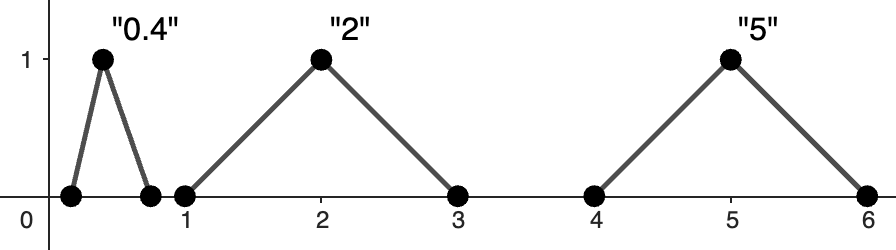
\includegraphics[width=0.5\linewidth]{images/division.png}
                \end{figure}
        \end{itemize}
    \end{example}
    
    From fuzzy arithmetic is also possible to define fuzzy functions, fuzzy integrals and fuzzy derivatives. In general, fuzzy numbers are used 
    to represent approximation.

    \section{Fuzzy measure and probability assignment}
    \begin{definition}
        If a field has the property that, if the sets $A_1, \dots ,A_n$ belong to the fields, then also the union and the intersection of the sets
        belong to the field, this is named a \emph{Borel field}. A function $g$ defined on a Borel field $B$ of the universe of discourse $X$ is 
        a \emph{fuzzy measure} if it has the following properties: 
        \begin{enumerate}
            \item $g(\varnothing)=0$ and $g(X)=1$.
            \item If $A,B \in B$ and $A \subseteq B$, then $g(A) \leq g(B)$.
            \item If $A_n \in B$ and $A_1 \subseteq A_2 \subseteq \dots$ then $\lim_{n \to \infty}g(A_n)=g(\lim_{n \to \infty}A_n)$.
        \end{enumerate}
    \end{definition}
    The fuzzy measure is different from classical measure, since the additivity property is relaxed.
    \begin{definition}
        The \emph{basic probabilistic assignment} is defined as:
        \begin{itemize}
            \item $m:\mathcal{P}(X) \rightarrow [0,1]$.
            \item $m(\varnothing)=0$.
            \item $\sum_{A \in \mathcal{P}(X)}m(A)=1$.
        \end{itemize}
        Where $m$ gives, for any set $A$ belonging to the power set of $X(\mathcal{P}(X))$, how much the available and relevant evidence
        supports the fact that a given element belongs to $A$.
    \end{definition}
    Note that: it is not needed that $m(X)=1$, it is not needed that $m(A) \leq m(B)$ when $A\subseteq B$ and no relationship holds between 
    $m(A)$ and $m(\lnot A)$. 

    \section{Evidence theory}
    We would like to define a measure of evidence for or against a proposition. To do that we will use two fuzzy measures: Belief and Plausibility.

    \begin{definition}
        \emph{Belief} is an estimation of the minimum probability that can be assigned to an element, given the collected evidence. The 
        \emph{Belief} has the following definition:
        \begin{itemize}
            \item $Bel:\mathcal{P} (X) \rightarrow [0,1]$.
            \item $Bel(\varnothing)=0$ and $Bel(X)=1$.
            \item $Bel(A_1 \cup A_2 \cup \dots \cup A_n) \geq \sum_{j}Bel(A_j)-\sum_{j<k}Bel(A_j \cap A_k)+\dots+(-1)^{n+1}Bel(A_1 \cap A_2 \cap \dots \cap A_n)$
            \item $Bel(A)+Bel(\lnot A) \leq 1$.
        \end{itemize}
    \end{definition}
    \begin{definition}
        \emph{Plausibility} is an estimation of the maximum probability that can be assigned to an element, given the collected evidence.
        The \emph{Plausibility} has the following definition:
        \begin{itemize}
            \item $Pl:\mathcal{P} (X) \rightarrow [0,1]$.
            \item $Pl(\varnothing)=0$ and $Pl(X)=1$.
            \item $Pl(A_1 \cap A_2 \cap \dots \cap A_n) \geq \sum_{j}Pl(A_j)-\sum_{j<k}Pl(A_j \cup A_k)+\dots+(-1)^{n+1}Pl(A_1 \cup A_2 \cup \dots \cup A_n)$
            \item $Pl(A)+Pl(\lnot A) \geq 1$.
        \end{itemize}
    \end{definition}
    The evidence theory can be used when we have multiple sources of knowledge and when the basic probability assignment is distributed on 
    different sets of statements, or intervals. In these cases, we may exploit the features of evidence theory to collect the basic probability
    assignments and to combine them to evaluate upper and lower bounds for probability of a single statement. Evidence theory has the following 
    implications: 
    \begin{itemize}
        \item It is not necessary to elicit a precise measurement from a knowledge source or an experiment if it is not realistic or feasible 
            to do so.
        \item The principle of insufficient reason is not imposed. Statements can be made about the likelihood of multiple events together without
            having to resort to assumptions about the probabilities of the individual events under ignorance.
        \item The axiom of additivity is not imposed. The measures can:
            \begin{itemize}
                \item Add to exactly one: it corresponds to a traditional probabilistic representation. 
                \item Add to less than one (sub-additive case): incompatibility between multiple sources of information providing conflicting 
                    information.
                \item Add to more than one (super-additive): cooperative effect between multiple sources of information (multiple sensors 
                    providing the same information).
            \end{itemize}
    \end{itemize}
    Given five sources ($A,B,C,D,E$ where $A$ is the target) of information it is possible to have four cases:
    \begin{itemize}
        \item Conflict: each source provides evidence for disjoint sets. 
            \begin{figure}[H]
                \centering
                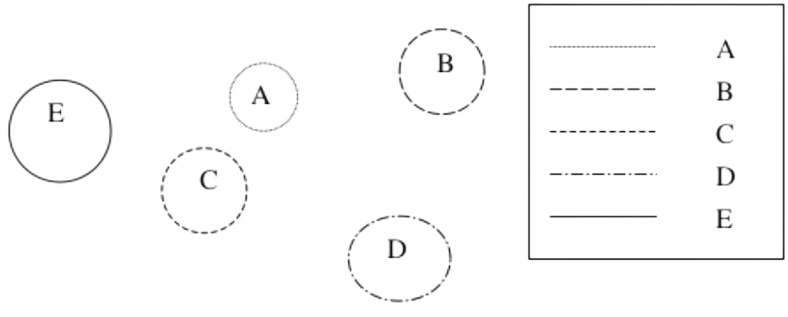
\includegraphics[width=0.5\linewidth]{images/conflict.png}
            \end{figure}
        \item Consonance: sources provide some evidence on nested sets converging on the target
            \begin{figure}[H]
                \centering
                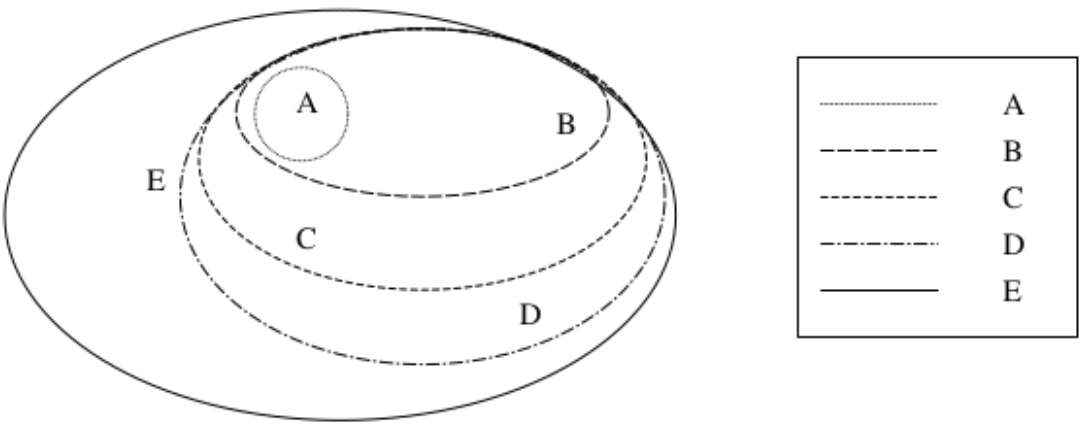
\includegraphics[width=0.5\linewidth]{images/consonance.png}
            \end{figure}
        \item Arbitrary: each source provides evidence for sets, only some of which include the target hypothesis. 
            \begin{figure}[H]
                \centering
                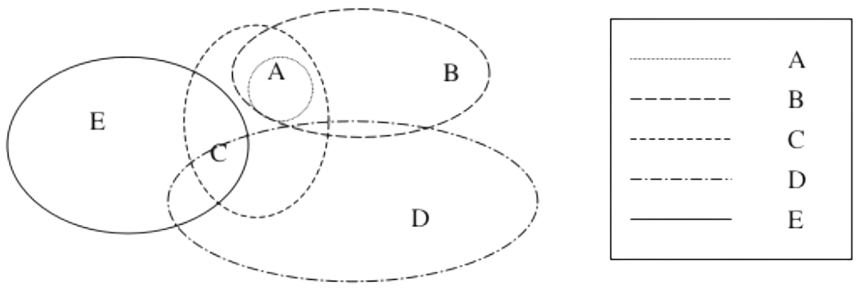
\includegraphics[width=0.5\linewidth]{images/arbitrary.png}
            \end{figure}
        \item Consistent: all sources provide some evidence for sets that include the same hypothesis. 
            \begin{figure}[H]
                \centering
                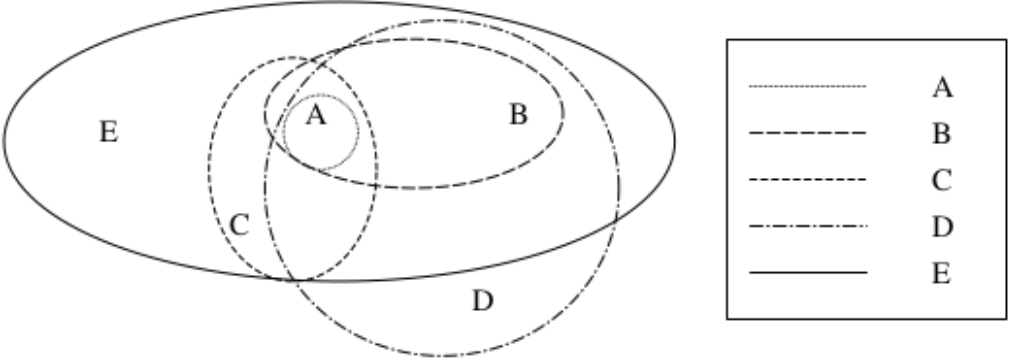
\includegraphics[width=0.5\linewidth]{images/consistent.png}
            \end{figure}
    \end{itemize}
    To combine the basic probability assignments it is possible to use the Dempster rule of combination:
    \[m_{1,2}(A)=\frac{\sum_{B \cap C=A}m_1(B)m_2(C)}{1-K}\]
    where $K$ is the basic probability mass associated with conflict. Its role in the denominator has the effect of completely ignoring conflict 
    and attributing any probability mass associated with conflict to the null set. The value of this variable is the following: 
    \[K=\sum_{B \cap C=O}m_1(B)m_2(C)\]
    \begin{example}[Klir, Yuan, 1995]
        Let’s assume that an old painting was discovered which strongly resembles paintings by Raphael. Such a discovery is likely to generate 
        various questions regarding the status of the painting. Let’s assume the following three questions:
        \begin{enumerate}
            \item Is the discovered painting a genuine painting by Raphael?
            \item Is the discovered painting a product of one of Raphael's many disciples?
            \item Is the discovered painting a counterfeit?
        \end{enumerate}
        Let $R$, $D$, and $C$ denote subsets of our universal set $X$-the set of all paintings, which contain the set of all paintings by Raphael, 
        the set of all paintings by disciples of Raphael, and the set of all counterfeits of Raphael's paintings, respectively.
        Assume now that two experts performed careful examinations of the painting and subsequently provided us with basic assignments $m_1$ and 
        $m_2$. By applying the above introduced formulas, it is possible to compute plausibility and belief of all the subsets of hypotheses.
    \end{example}

    \section{Possibility and necessity}
    \begin{definition}
        \emph{Possibility} is another fuzzy measure working on sets. A \emph{possibility measure} is given by the equation $\Pi : \mathcal{P}(X) \rightarrow [0,1]$,
        for which the following properties hols: 
        \begin{enumerate}
            \item $\Pi(\varnothing)=0$ and $\Pi(X)=1$.
            \item $A \subseteq B \implies \Pi(A) \leq \Pi(B)$. 
            \item $\Pi(A)=\sup_{x \in A} f(x)$ where $A \subset X$. 
        \end{enumerate}
    \end{definition}
    It can be uniquely defined by a possibility relationship $f:X \rightarrow [0,1]$ so that:
    \[\Pi\left(\bigcup_{i \in I}A_i\right)=\sup_{i \in I}\Pi\left(A_i\right)\]
    Therefore, $f$ is defined as $\Pi\left(\{X\}\right) \: \forall x \in X$.
    \begin{example}[Possibility]
        Given the set $x=\{0,1,2,3,4,5,6,7,8,9,10\}$ and $\Pi({x})$, the possibility that $x$ is close to the value $8$:
        \begin{center}
            \begin{tabular}{ | c | c | c | c | c | c | c | c | c | c | c | c | } 
            \hline
                $x$ & 0 & 1 & 2 & 3 & 4 & 5 & 6 & 7 & 8 & 9 & 10 \\ 
            \hline
                $\Pi\left(\{X\}\right)$ & 0 & 0 & 0 & 0 & 0 & 0.1 & 0.5 & 0.8 & 1 & 0.8 & 0.5 \\ 
            \hline
            \end{tabular}
        \end{center}
        Now we need to compute $\Pi(A)$ that is the possibility that $A$ includes an integer close to $8$.
        For a given set $A=\{2,5,9\}$, it is possible to compute its possibility: 
        \[\Pi(A)=\sup \left[\Pi\left(\{2\}\right), \Pi\left(\{5\}\right), \Pi\left(\{9\}\right)\right]=\sup\left[0,0.1,0.8\right]=0.8\]
    \end{example}

    \begin{definition}
        \emph{Necessity} is the dual of possibility, and it is defined as: 
        \[\Pi(A)=\-N(\lnot A)\]
        \emph{Necessity} also satisfy the condition: 
        \[\min\left[N(A),N(\lnot A)\right]=0\]
    \end{definition}
    
    Those two parameters are connected by the following relations: 
    \begin{itemize}
        \item $\Pi(A) \geq N(A)$.
        \item $N(A) > 0 \implies \Pi(A)=1$.
        \item $\Pi(A) < 1 \implies N(A)=0$.
    \end{itemize}
    \begin{definition}
        The \emph{confirmation degree} is a value that puts together possibility and necessity:
        \[C(A)=N(A)+\Pi(A)-1\]
        Negatives values of $C(A)$ correspond to a disconfirmation degree. 
    \end{definition}

    It is possible to demonstrate that if the focal set of elements of possibility (the one with values of $m$ different from $0$) is composed of sets with a single element,
    then $Bel$ and $Pl$ have the same value and this is equal to the sum of the probabilities of the elements of the set $A$ to which they are applied, given by $m$.

    The evidence in the probabilistic model is on single elements, in the possibility model it can also be on sets.

    Both have distribution functions, even if they are normalized differently: probabilities add up to one, for possibilities the maximum value is one.

    In possibility theory ignorance is expressed by assigning all the evidence to the total set (i.e., anything is possible), in probability, instead, by distributing a 
    uniform fraction of the evidence to each element (each element is equiprobable). 
    \begin{figure}[H]
        \centering
        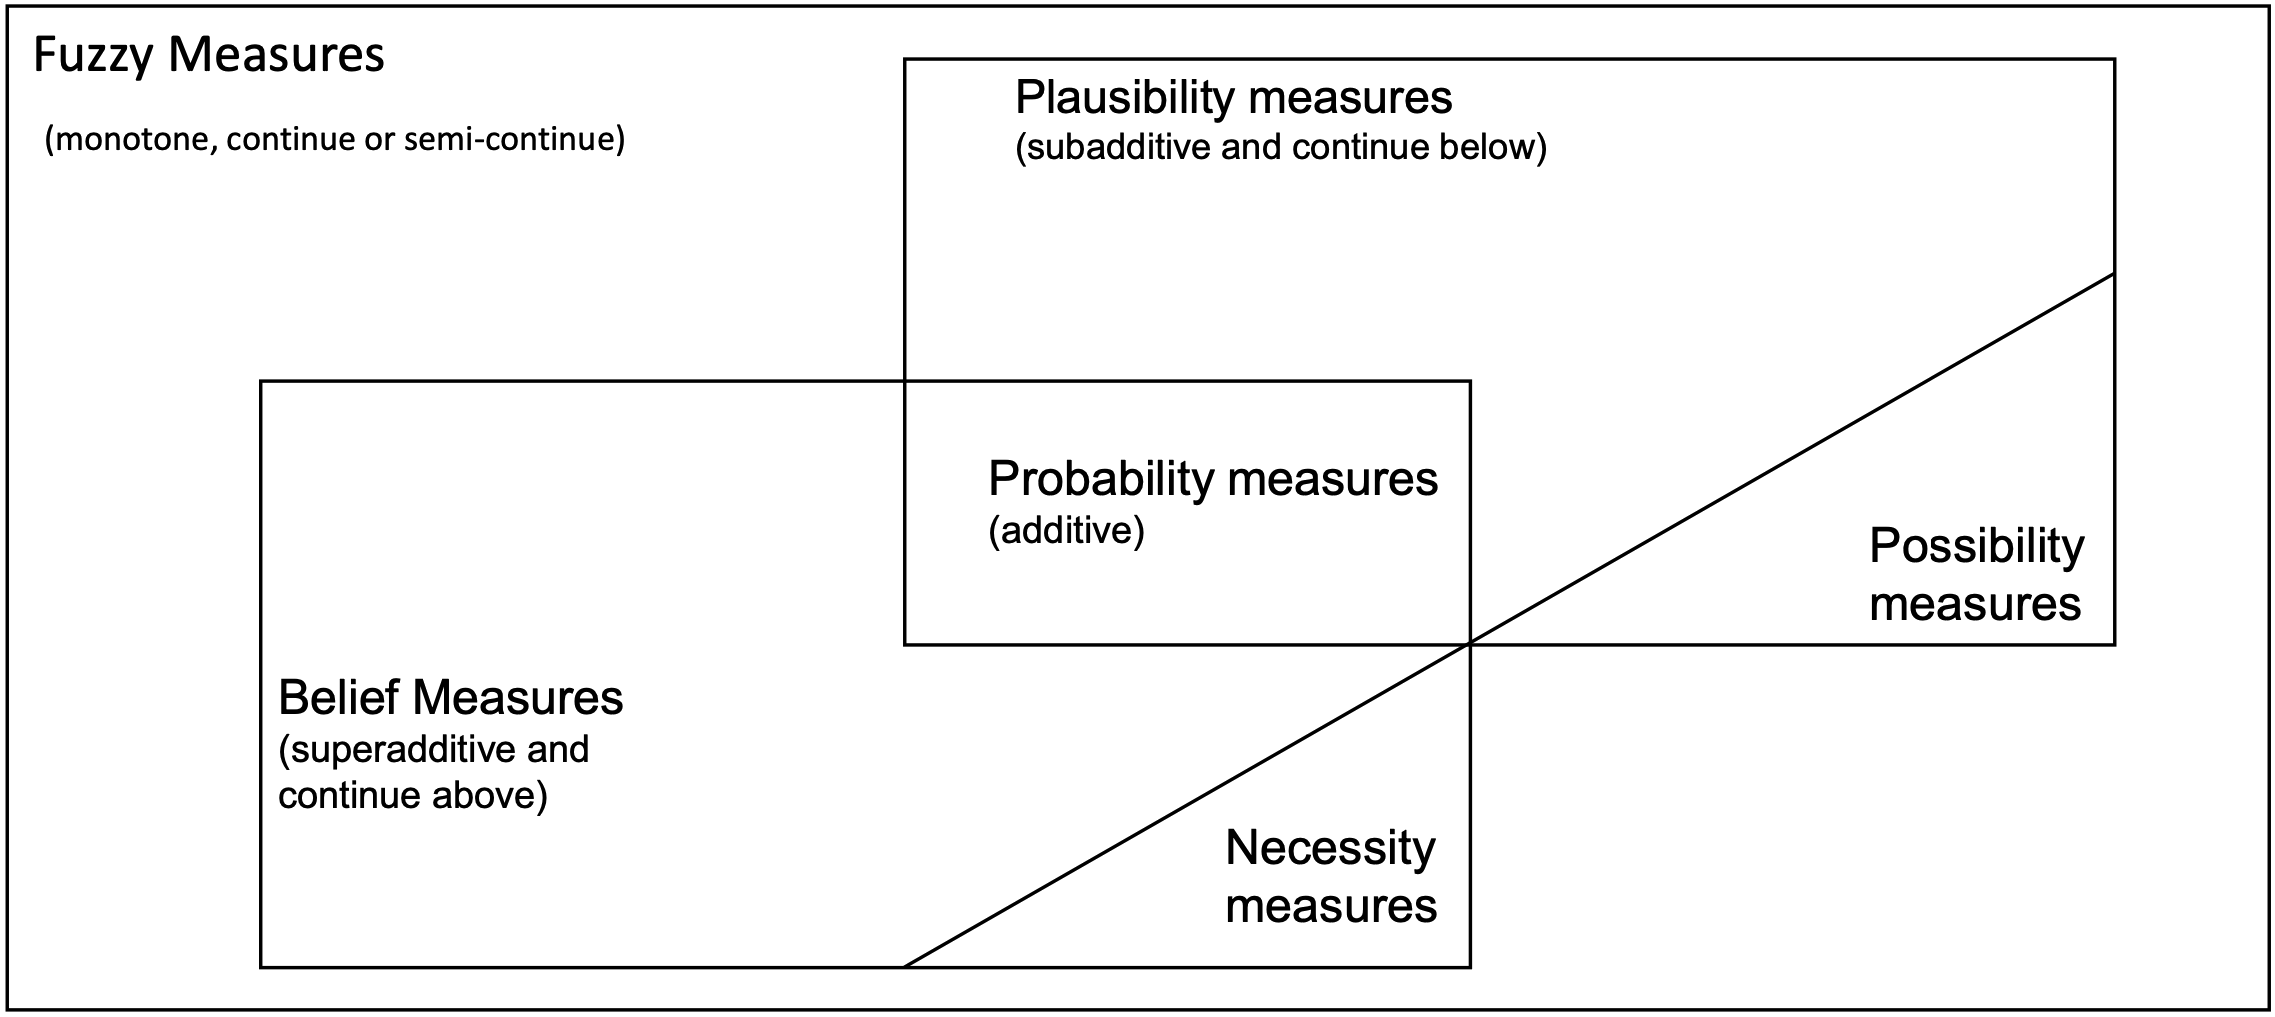
\includegraphics[width=0.75\linewidth]{images/measures.png}
        \caption{Inclusion relationships among fuzzy}
    \end{figure}

    \section{Fuzzyness measure}
    The fuzzyness measures provide the fuzzyness degree of a fuzzy set. A fuzzyness measure is the entropy of a fuzzy set. 
    \begin{definition}
        Given a fuzzy set $A=\{x,\mu_A(x)\}$ the fuzzyness measure (entropy) is defined as:
        \[d(A)=K \sum_{i=1}^{n}S(\mu_A(x_i))\]
        where $S(x)$ is the Shannon's function: 
        \[S(x)=-x \ln(x)-(1-x)\ln(1-x)\]
    \end{definition}
    \begin{example}
        Let's define $A$ as "the set of integer close to ten" we have that:
        \begin{center}
            \begin{tabular}{ | c | c | c | c | c | c | c | c | } 
            \hline
                $x$ & 7 & 8 & 9 & 10 & 11 & 12 & 13 \\ 
            \hline
                $\mu_A(x)$ & 0.1 & 0.5 & 0.8 & 1 & 0.8 & 0.5 & 0.1 \\ 
            \hline
            \end{tabular}
        \end{center}
        The entropy of this set has a value of: 
        \[d(A)=0.325+0.693+0.673+0.501+0+0.501+0.693+0.325=3.711\]
        Let's define $B$ as "the set of integer quite close to ten" we have that:
        \begin{center}
            \begin{tabular}{ | c | c | c | c | c | c | c | c | c | c | } 
            \hline
                $x$ & 6 & 7 & 8 & 9 & 10 & 11 & 12 & 13 & 14 \\ 
            \hline
                $\mu_A(x)$ & 0.1 & 0.3 & 0.4 & 0.7 & 1 & 0.8 & 0.5 & 0.3 & 0.1 \\ 
            \hline
            \end{tabular}
        \end{center}
        The entropy of this set has a value of: 
        \[d(A)=4.35\]
        It is possible to notice that $B$ is more fuzzy than $A$, since $d(B)>d(A)$.    
    \end{example}
    
\newpage

\chapter{Probabilistic reasoning}
    \section{Basic probability}
    \begin{definition}
        $A$ is a \emph{boolean-valued random variable} if $A$ denotes an event, and there is some degree of uncertainty as to whether $A$ occurs.

        \emph{Probability} of $A$ is the fraction of possible worlds in which $A$ is true. 
    \end{definition}
    \begin{theorem}[probabilty axioms]
        The axioms of the probability theory are: 
        \begin{itemize}
            \item $0 \leq P(A) \leq 1$. 
            \item $P(A=true) = 1 \: \land P(A=false) = 0\: $. 
            \item $P(A \lor B)=P(A)+P(B)-P(A \land B)$.
        \end{itemize}
    \end{theorem}
    Some useful formulas are: 
    \begin{enumerate}
        \item $P(\overline{A})=1-P(A)$.
        \item $P(A)=P(A \land B)+P(\overline{A} \land B)$
    \end{enumerate}
    \begin{definition}
        A \emph{multivalued random variable} $A$ is a random variable of arity $k$ if it can take on exactly one values out of $\{v_1,v_2,v_3,\dots,v_k\}$.
    \end{definition}
    \begin{theorem}[multivalued random variable axioms]
        The axioms for multivalued random variable are: 
        \begin{itemize}
            \item $P(A=v_i \land A=v_j) \:\:\:\:\:\: i \neq j$. 
            \item $P(A=v_1 \lor A=v_2 \lor A=v_3 \lor \dots \lor A=v_k)=1$. 
        \end{itemize}
    \end{theorem}
    Some useful formulas are: 
    \begin{enumerate}
        \item $P(A=v_1 \lor A=v_2 \lor \dots \lor A=v_i)=\sum_{j=1}^{i}{P(A=v_j)}$.
        \item $\sum_{j=1}^{k}{P(A=v_j)}=1$. 
        \item $P(B \land (A=v_1 \lor A=v_2 \lor \dots \lor A=v_i))=\sum_{j=1}^{i}{B \land A=v_j}$. 
        \item $P(B)=\sum_{j=1}^{k}{P(B \land A=v_j)}$.
    \end{enumerate}
    \begin{definition}
        The \emph{conditional probability} of $A$ given $B$ is the fraction of possible worlds in which $B$ is true that also have $A$ true. 
    \end{definition}
    The inference can be obtained using these formulas: 
    \begin{itemize}
        \item Chain rule: $P(A \land B)=P(A|B)P(B)$
        \item Bayes theorem: $P(A|B)=\dfrac{P(B|A)P(A)}{P(B)}$.
        \item Sum rule (marginalization): $P(A)=\sum_{b}{(A \land B=b)}$.
    \end{itemize}
    \begin{definition}
        Assume $A$ and $B$ are boolean random variables; $A$ and $B$ are independent (denote it with $A \perp B$) if and only if:
        \[P(A|B)=P(A)\]

        Given two random variables $A$ and $B$, the \emph{joint distribution} of $A$ and $B$ is the distribution of $A$ and $B$ together: $P(A,B)$
    \end{definition}
    It is possible to represent a joint distribution of $M$ (binary) variables with the following steps:
    \begin{itemize}
        \item Make a truth table listing all combination of values ($2^M$ entries).
        \item For each combination compute how probable it is. 
        \item Check that all probabilities sum up to one. 
    \end{itemize}

    \section{Probabilistic reasoning}
    Graphical models describe a factorization for the join distribution, and the process which possibly generates the data. They can be used for backward reasoning via Bayes' theorem.
    These models are graph-based algorithms for calculation and computation. The graphs can be: 
    \begin{itemize}
        \item Directed graphs (useful for designing models).
        \item Undirected graphs (good for some domains).
        \item Factor graphs (useful for inference and learning).
    \end{itemize}
    \begin{example}
        A fiendish murder has been committed. There are two suspects: the butler and the cook. There are three possible murder weapons: a butcher's knife, a pistol, and a 
        fireplace poker. 

        We know that the butler has served family well for many years, and the cook, hired recently, rumors of dodgy history, so we can say that: 
        \[P(Culprit=butler)=20\% \:\:\:\:\:\:\:\:\:\:\:\: P(Culprit=cook)=80\%\]
        Culprit is a binary random variable which probabilities add to $100\%$. 

        The butler is ex-army, and keeps a gun in a locker drawer. The cook has access to a lot of knives. The butler is older, and getting frail. We know that the weapons are: 
        \[Weapon=\{pistol,knife,poker\}\]
        And given the evidence we can state that: 
        \[P(Weapon|Culprit=butler)=\begin{bmatrix} 80\% & 10\% & 10\% \end{bmatrix}\]
        \[P(Weapon|Culprit=cook)=\begin{bmatrix} 5\% & 65\% & 30\% \end{bmatrix}\]
        
        Using the chain rule we can finally compute the joint distribution, that is: 
        \begin{table}[H]
            \centering
            \begin{tabular}{c|ccc|}
            \cline{2-4}
                                                  & \textbf{pistol} & \textbf{knife} & \textbf{poker} \\ \hline
            \multicolumn{1}{|l|}{\textbf{cook}}   & $4\%$           & $52\%$         & $24\%$         \\
            \multicolumn{1}{|l|}{\textbf{butler}} & $16\%$          & $2\%$          & $2\%$          \\ \hline
            \end{tabular}
        \end{table}

        Using the sum rule we can compute the marginal distribution of culprits: cook ($80\%$), and butler ($20\%$). 
        And the marginal distribution of weapons: pistol ($20\%$), knife ($54\%$), and poker ($26\%$). 
        If at a certain point we discover the weapon, we can use the Bayes' theorem to compute who is the culprit. 
    \end{example}

    \section{Density estimation and its complexity}
    To compute the probability for logic expression we can use the sum: 
    \[P(E)=\sum_{row \backsim E}P(row)\]
    To compute the inference (that is probabilistic reasoning) we can use the formula: 
    \[P(E_1|E_2)=\dfrac{P(E_1 \land E_2)}{E_2}=\dfrac{\sum_{row \backsim E_1 \land E_2}P(row)}{\sum_{row \backsim E_2}P(row)}\]
    \begin{example}
        Given the following truth table: 
        \begin{table}[H]
            \centering
            \begin{tabular}{|c|c|c|c|}
            \hline
            $A$ & $B$ & $C$ & $P(A,B,C)$ \\ \hline
            0   & 0   & 0   & 0.30       \\ \hline
            0   & 0   & 1   & 0.05       \\ \hline
            0   & 1   & 0   & 0.10       \\ \hline
            0   & 1   & 1   & 0.05       \\ \hline
            1   & 0   & 0   & 0.05       \\ \hline
            1   & 0   & 1   & 0.10       \\ \hline
            1   & 1   & 0   & 0.25       \\ \hline
            1   & 1   & 1   & 0.10       \\ \hline
            \end{tabular}
        \end{table}
        $P(A)$ can be found by summing all the probability where $A=1$, that is: 
        \[P(A) = 0.05 + 0.10 + 0.25 + 0.10 = 0.5\]
        $P(A \land B)$ can be found by summing all the probability where $A=1$ and $B=1$, that is: 
        \[P(A \land B) = 0.25 + 0.10 = 0.35\]
        $P(\overline{A} \lor B)$ can be found by summing all the probability where $A=0$ or $B=1$, that is: 
        \[P(\overline{A} \lor B) = 0.30 + 0.05 + 0.10 + 0.05 + 0.25 + 0.10 = 0.85\]
        $P(A | B)$ can be found by dividing the probability of $A=1$ and $B=1$ by the probability where $B=1$, that is: 
        \[P(A | B) = \dfrac{(0.25+0.10)}{(0.10+0.05+0.25+0.10)}=0.7\]
        $P(C | A \land B)$ can be found by dividing the probability of $A=1$ and $B=1$ and $C=1$ by the probability where $A=1$ and $B=1$, that is: 
        \[P(C | A \land B) = \dfrac{(0.10)}{(0.25+0.10)}=0.285\]
        $P(\overline{A} | C)$ can be found by dividing the probability of $A=0$ and $C=1$ by the probability where $C=1$, that is: 
        \[P(\overline{A} | C) = \dfrac{(0.05+0.05)}{(0.05+0.05+0.10+0.10)}=0.333\]
    \end{example}
    \begin{definition}
        A \emph{density estimator} learns a mapping from a set of attributes to a probability distribution over the attributes space: 
        \[M:\{0,1\}^I \rightarrow [0,1]\]
    \end{definition}
    We can use likelihood for evaluating density estimation. Given a record $x$, a density estimator $M$ tells you how likely it is $\widehat{P}(x|M)$. Given a dataset with $N$ 
    records, a density estimator can tell how likely data is under the assumption that all records were independently generated from it: 
    \[\widehat{P}(\textnormal{dataset})=\widehat{P}(x_1,x_2,\dots,x_N)=\prod_{n=1}^{N}\widehat{P}(x|M)\]
    Since likelihood can get too small we usually use log-likelihood:
    \[\log{\widehat{P}(\textnormal{dataset})}=\log{\prod_{n=1}^{N}{\widehat{P}(x_n|M)}}=\sum_{n=1}^{N}{\log{\widehat{P}(x_n|M)}}\]
    Density estimators can do many good things: sort the records by probability, and thus spot weird records, inference and can be used for Bayes classifiers. 
    The main problem about joint density estimators is that they can badly overfit. 

    The naïve Bayes estimator model assumes that each attribute is distributed independently of the other attributes. Let $x[i]$ denote the $i^{th}$ field of record $x$, the naïve
    density estimator says that: 
    \[x[i] \perp \{x[1],x[2],\dots,x[i-1],x[i],x[i+1],\dots,x[I]\}\]
    It is important to know that all attributes are equally important and that knowing one attribute says nothing about the value of another. This last assumption is almost never
    correct, but works quite well when used in practice. 
    \begin{example}
        Given four variables $A,B,C,D$. For the naïve Bayes estimator model they are all independent thanks to the assumptions. This means that: 
        \[P(A,\overline{B},C,\overline{D}) = P(A)P(\overline{B})P(C)P(\overline{D})\]
    \end{example}
    To learn a naïve Bayes estimator we have to suppose that $x[1],x[2],\dots,x[n]$ are independently distributed. We can construct any row of the implied joint distribution on 
    demand with the formula: 
    \[\widehat{P}(x[1]=u_1,x[2]=u_2,\dots,x[I]=u_I) = \prod_{k=1}^{I} \widehat{P}(x[k]=u_k)\]
    And we can do inference.
    \begin{table}[H]
        \centering
        \begin{tabular}{c|c|c|}
        \cline{2-3}
                                                   & \textbf{Joint estimator} & \textbf{Naïve estimator} \\ \hline
        \multicolumn{1}{|c|}{\textbf{Modelling}}   & Anything                 & Boring distributions     \\ \cline{1-1}
        \multicolumn{1}{|c|}{\textbf{Attributes}}  & Few Boolean              & Many multivalued         \\ \cline{1-1}
        \multicolumn{1}{|c|}{\textbf{Overfitting}} & Yes                      & Quite robust             \\ \hline
        \end{tabular}
    \end{table}
    \begin{figure}[H]
        \centering
        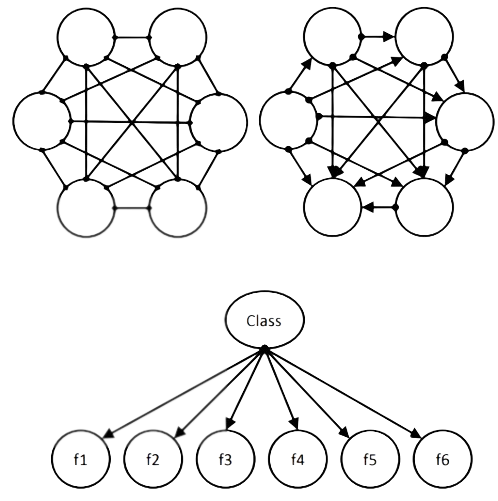
\includegraphics[width=0.75\linewidth]{images/naive-joint.png}
        \caption{Comparison between a joint and a naïve estimator}
    \end{figure}

\newpage

\chapter{Graphical models}
    \section{Introduction}
    In the real world the random variables are usually correlated. So, to overcome this problem we can describe a probability distribution via: 
    \begin{itemize}
        \item Conditional independence assumptions that apply on a subset of them. 
        \item A set of conditional probabilities with their priors. 
    \end{itemize}
    These models are called graphical models. 

    \section{Bayesian network}
    A Bayesian network is a method to describe the joint probability distribution of a set of variables. It can be represented as a 
    directed graph where the nodes represent random variables and the edges represent direct influence. 
    \begin{example}
        Given the following Bayesian network:
        \begin{figure}[H]
            \centering
            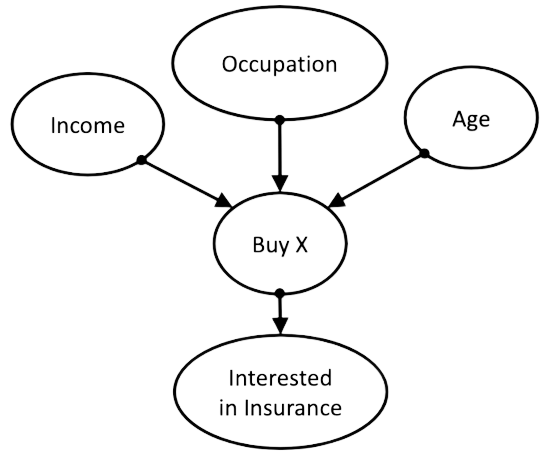
\includegraphics[width=0.4\linewidth]{images/insurance.png}
        \end{figure}
        We can see that the random variables "age", "income", and "occupation" are independent while "buy X" and 
        "Interested in insurance" are conditional probability distributions. 
    \end{example}
    Let $x_1,x_2,\dots,x_n$ be a set of variables. We have that a Bayesian network can tell any combination probability. The full joint 
    distribution will require: 
    \[2^N-1 \textnormal{ parameters}\] 
    To represent the probabilities in the network we need only the priors and conditional parameters. We simply multiply the number of
    nodes for $2^k$, where $k$ is the number of incoming edges, and we obtain the numbers of parameters needed. 
    \begin{example}
        Given the following Bayesian network:
        \begin{figure}[H]
            \centering
            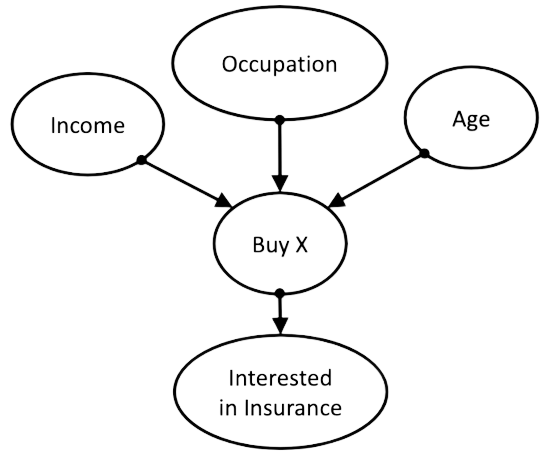
\includegraphics[width=0.4\linewidth]{images/insurance.png}
        \end{figure}
        In this case we have that the full joint distribution will need: 
        \[2^N-1=2^5-1=31 \textnormal{ parameters}\]
        And to represent the Bayesian network we will need 
        \[3 \cdot 2^0 + 1 \cdot 2^3 + 1+ \cdot 2^1 = 13 \textnormal{ parameters}\]
    \end{example}
    \begin{definition}
        We say $X_1$ is \emph{conditionally independent} of $X_2$ given $X_3$ if the probability of $X_1$ is independent of $X_2$ given some
        knowledge about $X_3$:
        \[P(X_1|X_2,X_3)=P(X_1|X_3)\]
    \end{definition}
    The same can be said for a set of variables: $X_1,X_2,X_3$ is independent of $Y_1,Y_2,Y_3$ given $Z_1,Z_2,Z_3$:
    \[P(X_1,X_2,X_3|Y_1,Y_2,Y_3,Z_1,Z_2,Z_3)=P(X_1,X_2,X_3|Z_1,Z_2,Z_3)\]
    \begin{example}
        Martin and Norman toss the same coin. Let be $A$ “Norman's outcome”, and $B$ “Martin's outcome”. Assume the coin might be biased; 
        in this case $A$ and $B$ are not independent: observing that $B$ is heads causes us to increase our belief in $A$ being heads. So
        it holds: 
        \[P(A|B) \neq P(A)\]
        Variables $A$ and $B$ are both dependent on $C$ “The coin is biased towards Heads with probability $\theta$”. Once we know for 
        $C$ then any evidence about $B$ cannot change our belief about $A$:
        \[P(A|B,C)=P(A|C)\]
    \end{example}
    \begin{definition}
        A \emph{prior probability} is a probability with zero incoming edges. 
    \end{definition}
    A node is independent of its ancestors given its parent. 
    \begin{example}
        The event “Grass is wet” ($W=true$) has two possible causes: either the water “Sprinkler” is on ($S=true$) or it is “Raining”
        ($R=true$). The related Bayesian network is the following.
        \begin{figure}[H]
            \centering
            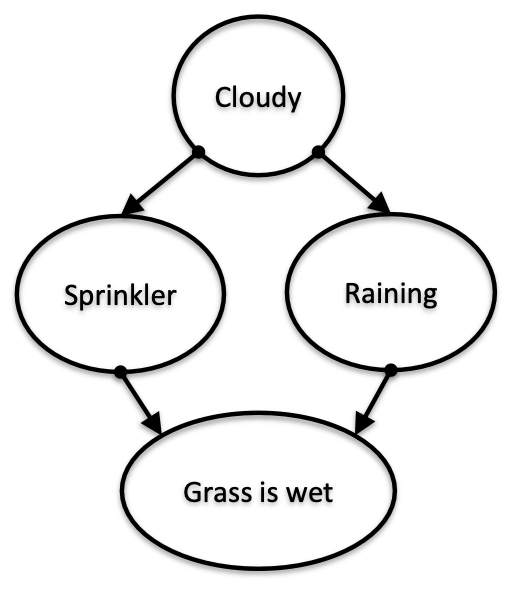
\includegraphics[width=0.4\linewidth]{images/sprinkler.png}
        \end{figure}
        Where the probabilities for cloudy are: 
        \begin{table}[H]
            \centering
            \begin{tabular}{c|cc|}
            \cline{2-3}
                                              & $true$ & $false$ \\ \hline
            \multicolumn{1}{|c|}{$P(cloudy)$} & 0.5    & 0.5     \\ \hline
            \end{tabular}
        \end{table}
        Where the probabilities for sprinkler are: 
        \begin{table}[H]
            \centering
            \begin{tabular}{c|cc|}
            \cline{2-3}
                                                 & $P(C)=true$ & $P(C)=false$ \\ \hline
            \multicolumn{1}{|c|}{$P(sprinkler)$} & 0.5         & 0.9          \\ \hline
            \end{tabular}
        \end{table}
        Where the probabilities for raining are: 
        \begin{table}[H]
            \centering
            \begin{tabular}{c|cc|}
            \cline{2-3}
                                               & $P(C)=true$ & $P(C)=false$ \\ \hline
            \multicolumn{1}{|c|}{$P(raining)$} & 0.5         & 0.2          \\ \hline
            \end{tabular}
        \end{table}
        Where the probabilities for the wet grass are: 
        \begin{table}[H]
            \centering
            \begin{tabular}{c|cccc|}
            \cline{2-5}
                                         & $S=t,R=t$ & $S=t,R=f$ & $S=f,R=t$ & $S=f,R=f$ \\ \hline
            \multicolumn{1}{|c|}{$P(W)$} & 0.99                      & 0.9                        & 0.9                       & 0                                 \\ \hline
            \end{tabular}
        \end{table}
        With all these values it is possible to compute all the probabilities. 
        \begin{figure}[H]
            \centering
            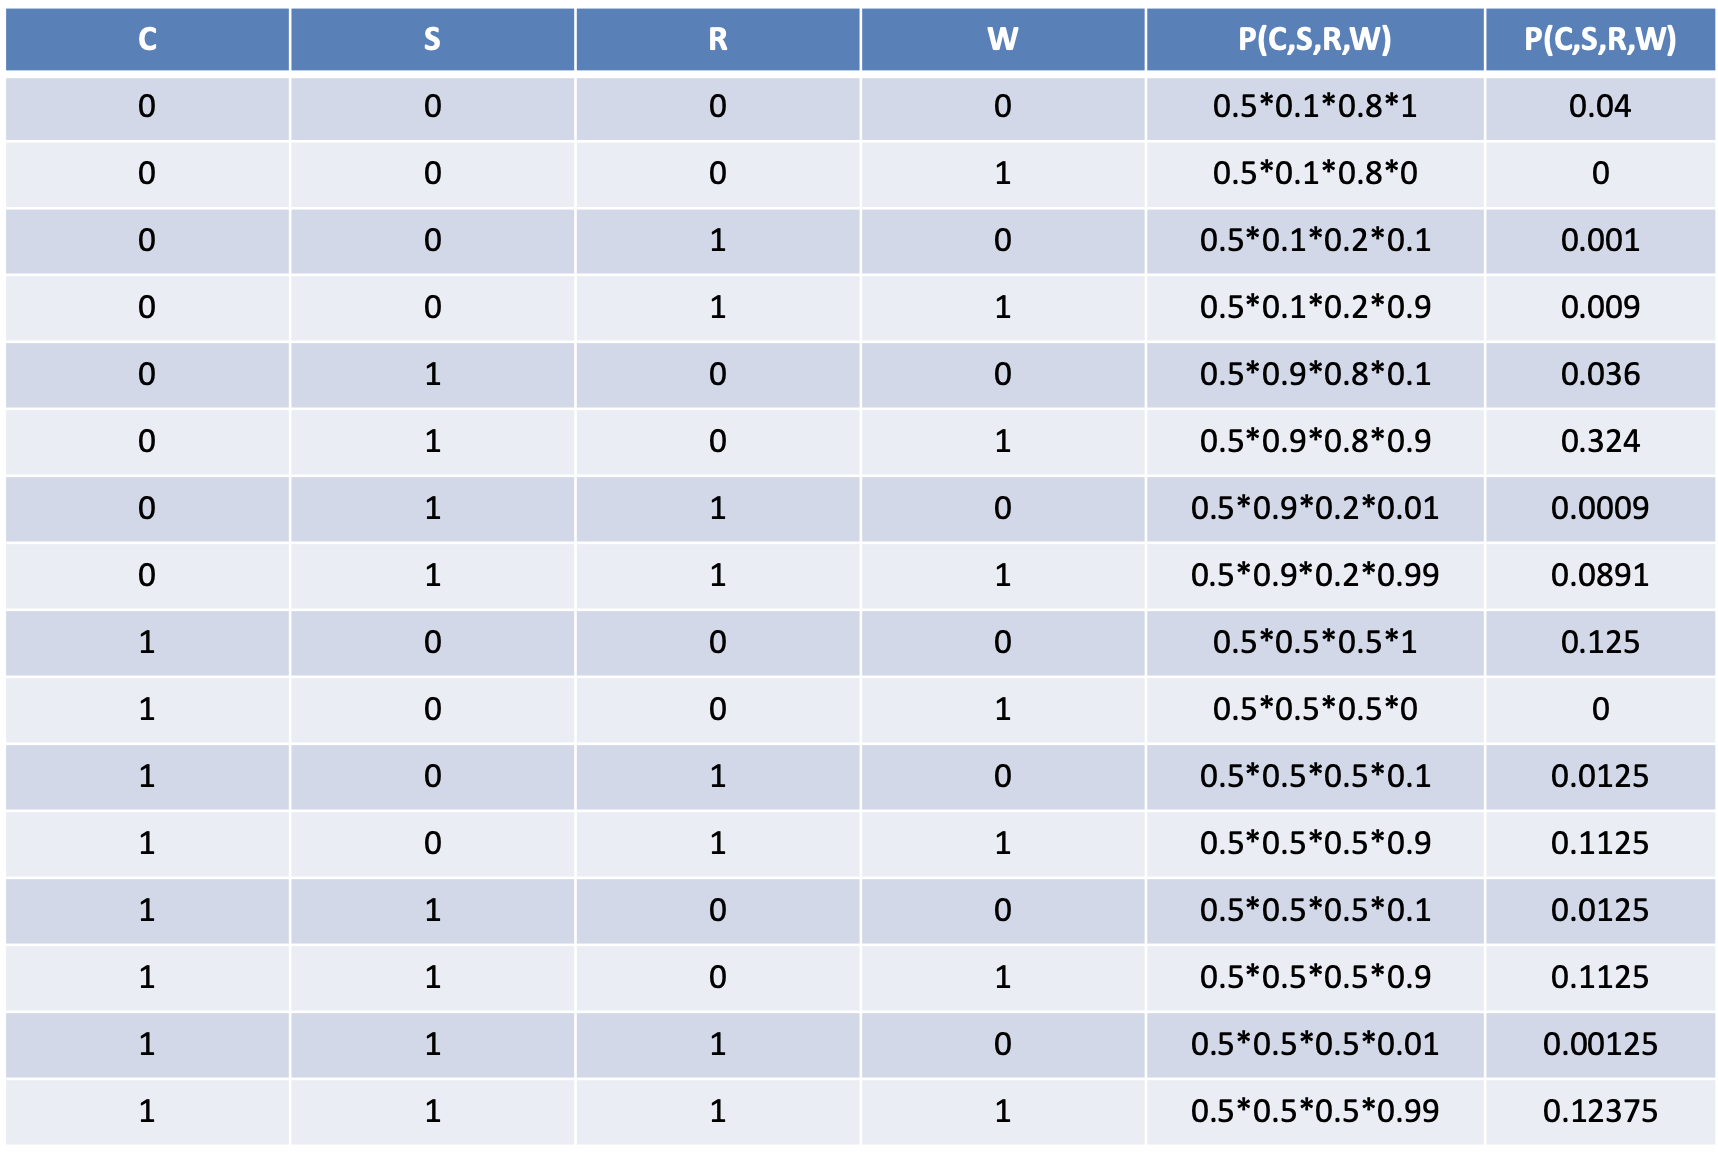
\includegraphics[width=0.9\linewidth]{images/probabilities.png}
        \end{figure}
    \end{example}
    Explaining away is known in statistics as Berkson's paradox, or selection bias, and it describes two variable which become dependent 
    because you observe a third one. In general, the independencies in a Bayesian network can be: 
    \begin{figure}[H]
        \centering
        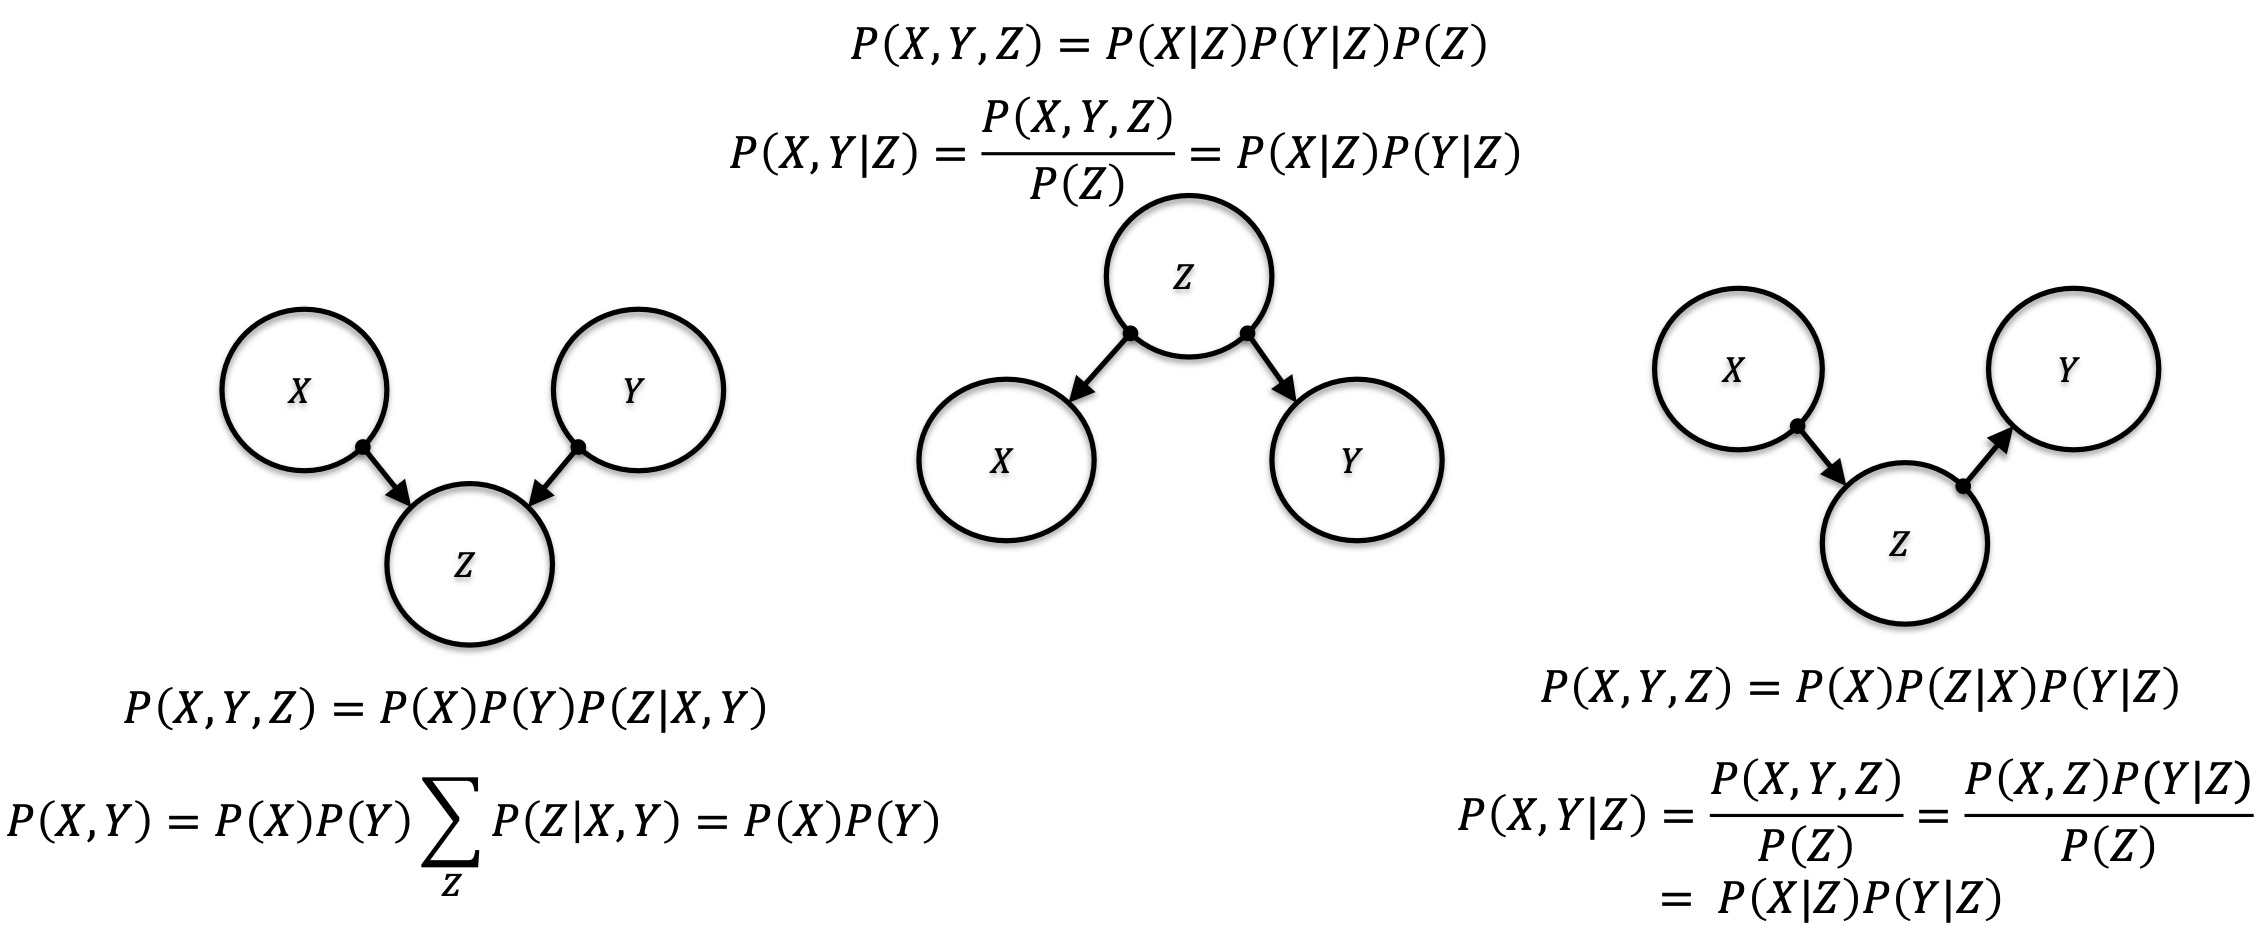
\includegraphics[width=1\linewidth]{images/independencies.png}
    \end{figure}


\end{document}